%pdflatex main.tex
\documentclass[12pt]{article}
\usepackage{natbib}
\usepackage[francais]{babel}
\usepackage{natbib}
\usepackage{url}
\usepackage[utf8x]{inputenc}
\usepackage{amsmath}
\usepackage{graphicx}
\usepackage{caption}
\usepackage{subcaption}
\usepackage{float}
\graphicspath{{images/}}
\usepackage{amsthm}
\usepackage{parskip}
\usepackage{fancyhdr}
\usepackage{xfrac}
\usepackage{esvect}
\usepackage{vmargin}
\usepackage{gensymb}
\setmarginsrb{3 cm}{2.5 cm}{3 cm}{2.5 cm}{1 cm}{1.5 cm}{1 cm}{1.5 cm}

\title{Projet Quadtree}								% Title
\author{Groupe 2}								% Author
\date{\today}											% Date

\makeatletter
\let\thetitle\@title
\let\theauthor\@author
\let\thedate\@date
\makeatother

\pagestyle{fancy}
\fancyhf{}
\rhead{\theauthor}
\lhead{\thetitle}
\cfoot{\thepage}
\newtheorem*{rappel}{Rappel}
\newtheorem*{nota}{N.B}
\newtheorem*{req}{Remarque}
\begin{document}

%%%%%%%%%%%%%%%%%%%%%%%%%%%%%%%%%%%%%%%%%%%%%%%%%%%%%%%%%%%%%%%%%%%%%%%%%%%%%%%%%%%%%%%%%

\begin{titlepage}
	\centering
    \vspace*{0.5 cm}
    
\includegraphics[scale = 0.75 ]{logo1.png}\\[1.0 cm]	% University Logo
    \textsc{\LARGE EISTI}\\[2.0 cm]			% University Name
    \rule{\linewidth}{0.2 mm} \\[0.5 cm]
    { \huge \bfseries \thetitle}\\
    \rule{\linewidth}{0.2 mm} \\[1.5 cm]
	\textsc{\Large Algorithmique et programmation fonctionnelle}\\[0.5 cm]	% Course Code
	\textsc{\large CPI1 C2 - Groupe 2}\\[0.5 cm]		% Course Name
	
	\begin{minipage}{0.4\textwidth}
	\centering
		\begin{center} \large
		Amine TAGHROUT\\
		David RIGAUX \\
		Mehdi DALAA 
			\end{center}
			\end{minipage}~
			\begin{minipage}{0.4\textwidth}
	\end{minipage}\\[0.8 cm]
	{\large \thedate}\\[1 cm]
	\vfill
	
\end{titlepage}

%%%%%%%%%%%%%%%%%%%%%%%%%%%%%%%%%%%%%%%%%%%%%%%%%%%%%%%%%%%%%%%%%%%%%%%%%%%%%%%%%%%%%%%%%

\tableofcontents
\addtocontents{toc}{~\hfill\textbf{Page}\par}
\pagebreak

%%%%%%%%%%%%%%%%%%%%%%%%%%%%%%%%%%%%%%%%%%%%%%%%%%%%%%%%%%%%%%%%%%%%%%%%%%%%%%%%%%%%%%%%%

\section*{Introduction}
\addcontentsline{toc}{section}{\protect\numberline{}Introduction}
L\'objet de notre projet en informatique est de réaliser un programme pouvant manipuler des images encodées sous forme d\'arbre. Pour réaliser ce projet, nous avions un temps imparti d\'un mois, et le langage de programmation devait être le OCaml. Les images que nous devons traiter sont de type \textit{.ppm}. \par
Le \textit{portable pixmap file format} (PPM) est un format de fichier utilisé pour les  échanges. Il a été défini et est utilise par le projet NetPBM. Le format
de fichier est utilisé pour des images couleur. Chaque pixel est code par trois valeurs (rouge, vert et bleu). Le codage d\'une image en PPM est le suivant :
\begin{enumerate}
\item P3 (Numéro magique)
\item Largeur Hauteur (Dimensions)
\item MaxVal (Valeur maximum des couleurs)
\item Les données de l'image : succession des valeurs associées à chaque pixel
\end{enumerate}\par
Comme on l'avait fait remarquer, on ne s\'intersse qu'aux images carrées de taille $2^{n}*2^{n}$ une image unicolore se représente par sa couleur, tandis qu\'une image composite se divise naturellement en quatre sous-images carrées. \
Les feuilles d\'un \textit{quadtree} correspondent donc à une zone de l\'image ayant une couleur unique. Les nœuds internes stockent la moyenne des couleurs de leurs fils
\section{Étude du projet}
Tout d'abord et puisque une image ppm est représentée par des matrices (listes de listes) il fallait faire des manipulations sur des fichiers constitués de matrices.\
La première manipulation qu'on avait faite était de lire un fichier en utilisant la fonction \textit{readfile}. Cette dernière prend en paramètre un fichier et permet de le lire ligne par ligne. Cependant, le fichier lu peut éventuellement contenir des commentaires, des caractères spéciaux ou des espaces. C'est pour cela qu'on avait fait la fonction \textit{filtre} qui prend en paramètre une liste de string et qui enlève tous les éléments indésirables de façon à avoir à la fin un fichier qui ne contient que le nom, la taille de l'image et les suites de pixels.\
l'étape suivante était de créer une fonction qui permet de regrouper les pixels sous forme de triplets et pour cela on n'avait besoin que des pixels. C'est pour cela qu'on avait besoin de la fonction 
\textit{clean} qui enlève le titre et les dimensions de l'image de façon à ne garder que les pixels. A partir de ce moment, on pouvait utiliser la fonction regroupe qui prend en paramètre une liste de string et qui renvoie une liste de triplets d'entiers.\
On avait créer aussi des fonctions complémentaires comme \textit{superlecture} qui permets à l'utilisateur de lire et en même temps filtrer le fichier voulu. De plus, et comme on peut clairement le voir dans le quadtree, les nœuds internes stockent la moyenne des couleurs de leurs fils. C'est pour cela qu'une fonction moyenne était nécessaire mais avant cela il fallait créer un fonction qui calcule la somme des composantes des triplets de la liste des pixels et c'est ce que fait la fonction somme qui prend en paramètre une liste de triplet et qui renvoie le triplet
qui a pour composantes la somme de toutes les composantes.\
Comme vous pouvez le remarquez, la fonction moyenne prend en paramètre le triplet renvoyé par la fonction somme et la liste initiale et elle renvoie un triplet qui a comme composantes la moyenne de toutes les autres.\
Après cela, nous avons également fait des fonctions supplémentaires comme \textit{superlecture} qui permet de lire et de filtrer en même temps le fichier voulu, ou encore la fonction \textit{moyenne}
qui prend en paramètre le fichier initiale et qui renvoie directement la moyenne de pixels.\
La deuxième partie du projet consistait à créer le type \textit{quadtree} et biensûr créer l'arbre \textit{quadtree} en utilisant la fonction \textit{creerArbre}.Tous cela, pour pouvoir 
faire différentes manipulations et opérations sur l'image. Parmi ces opérations on trouve les simples et les complexes. \\

De plus, pour faciliter l'utilisation du programme codé, nous avons créé une interface graphique faite à l'aide de la libraire graphique \textit{LablGTK2}.
\section{LablGTK}
LablGTK est une interface OCaml du projet GTK+ 1.2 et 2.x. Cette librairie nous permet de créer des interfaces graphiques orienté-objets.
\subsection{GTK+}
\textbf{GTK+} (\textit{The \textbf{G}IMP \textbf{T}ool\textbf{k}it}) est un ensemble de bibliothèques logicielles, c'est-à-dire un ensemble de fonctions permettant de réaliser des interfaces graphiques. Cette bibliothèque a été développée originellement pour les besoins du logiciels de traitement d'image GIMP. GTK+ est maintenant utilisé dans de nombreux projets, dont les environnements de bureau \textit{GNOME}, \textit{Xfce}, \textit{Lxde} et \textit{ROX}. \\
GTK+ est un projet libre (licence GNU LGPL 2.1) et multiplateforme.
\section{Arbre Quadtree}
Qu'est ce qu'un arbre Quadtree et comment on l'a créé
\section{Fonction I/O}
Les fonctions I/O (\textit{In/Out}) dans notre projet sont indispensable pour pouvoir faire des manipulations d'images. Nous avons en tout quatres fonctions I/O que nous allons vous présenter dans les sous-parties suivantes. 
\subsection{Chargement}
Pour ce qui est du chargement, nous avons créé deux fonctions qui font deux opérations distinctes l'un de l'autre. \\
Sachant que nous ne pouvons pas stocker un arbre en OCaml nous avons donc décider de créer un fichier temporaire au moment où l'utilisateur fait le choix de l'image à modifier. En effet, cela nous permet donc de travailler avec l'image mais sans modifier l'image de départ et nous permet également ainsi de stocker les modifications. Donc nous travaillons principalement avec le fichier temporaire créer suite au chargement de l'image. \\
La deuxième fonction de chargement est la fonction qui nous permet de lire le fichier et de ressortir un arbre de type \textit{quadtree} pour faire ensuite les modifications en questions.
\subsection{Enregistrement}
Pour l'enregistrement, nous avons, comme pour le chargement, deux fonctions distincts. \\
Une fois le fichier chargé sous forme d'arbre et modifié nous avons fais une fonction qui ressort l'arbre dans le fichier temporaire pour pouvoir stocker l'opération faite à l'image.\\
La deuxième fonction, n'entre en jeu dès que l'on veut sauvegarder l'image et ressortir la version finale. L'utilisateur a la possibilité d'enregistrer-sous ou tout simplement d'écraser l'ancienne image en enregistrant. Commençons par expliquer la fonction permettant d'enregistrer. Sachant que nous travaillons avec un fichier temporaire, qui a toute les modifications déjà faite, il ne nous suffit qu'à supprimer l'image original et de renommer ensuite le fichier temporaire au nom de base. Cependant, nous recréons un fichier temporaire aussitôt pour laisser la possibilité à l'utilisateur de continuer à travailler sur son image. Maintenant pour ce qui est de l'enregistrement-sous, il y a la même logique que l'enregistrement simple, mais cette fois nous ne supprimons pas l'image de original. En effet, nous ne faisons que déplacer le fichier temporaire, en le renommant avec le nom que l'utilisateur souhaite. Si l'utilisateur ne mets pas l'extension \textit{.ppm} à la fin du nom de fichier souhaité, nous avons créé une petite fonction qui permet de faire la vérification et en cas d'absence de cette extension nous la rajoutons à la fin du nom au moment de renommer le fichier. De plus, comme pour l'enregistrement, nous créons aussitôt un autre fichier temporaire pour laisser la possibilité à l'utilisateur de continuer à travailler avec cette image.
\section{Fonctions de manipulation}
\subsection{Opérations Simples}
\subsubsection{Rotation de 90$^{\circ}$}
\begin{enumerate}
\item Rotation vers la droite : cette opération consiste à effectuer une rotation de l'image vers la droite. Pour cela, on a utilisé la fonction \textit{rotated} qui décale les fils d'une place vers la droite	
\item Rotation vers la gauche : cette opération consiste à effectuer une rotation de l'image vers la gauche. Pour cela, on a utilisé la fonction \textit{rotateg} qui décale les fils d'une place vers la gauche   
\end{enumerate}
\subsubsection{Miroir}
\begin{enumerate}
\item Miroir haut-bas : cette opération consiste à créer un arbre de façon à ce que les feuilles soient interverties de haut en bas. Par exemple : \\
		   $\begin{matrix}
		   1 & 2 \\
		   4 & 3
		   \end{matrix} \quad $\ devient\
		   $\quad \begin{matrix}
		   4 & 3 \\
		   1 & 2
		   \end{matrix}$
\item Miroir gauche-droite : cette opération consiste à créer un arbre de façon à ce que les feuilles soient interverties de haut en bas. Par exemple :  \\
		   $\begin{matrix}
		   1 & 2 \\
		   4 & 3
		   \end{matrix} \quad$ devient
		   $\quad  \begin{matrix}
		   2 & 1 \\
		   3 & 4
		   \end{matrix}$
\end{enumerate}
\subsubsection{Inversion}
Cette opération consiste à inverser les couleurs de l'image. Ce que fait la fonction inverse qui prend en paramètre le triplet représentant la moyenne des couleurs et qui renvoie le triplet dont les composantes sont la différence avec 255 qui est le maximum des pixels. 
\subsection{Opérations Avancées}
\subsubsection{Compression}
\subsubsection{Segmentation}
\section{Graphiques}
Pour pouvoir créer une bonne interface graphique, il nous a fallu penser à tout ce qu'un utilisateur aurait besoin d'avoir et à quel moment. Voici ce que l'utilisateur aperçoit dès l'ouverture de l'application :\\

\begin{center}
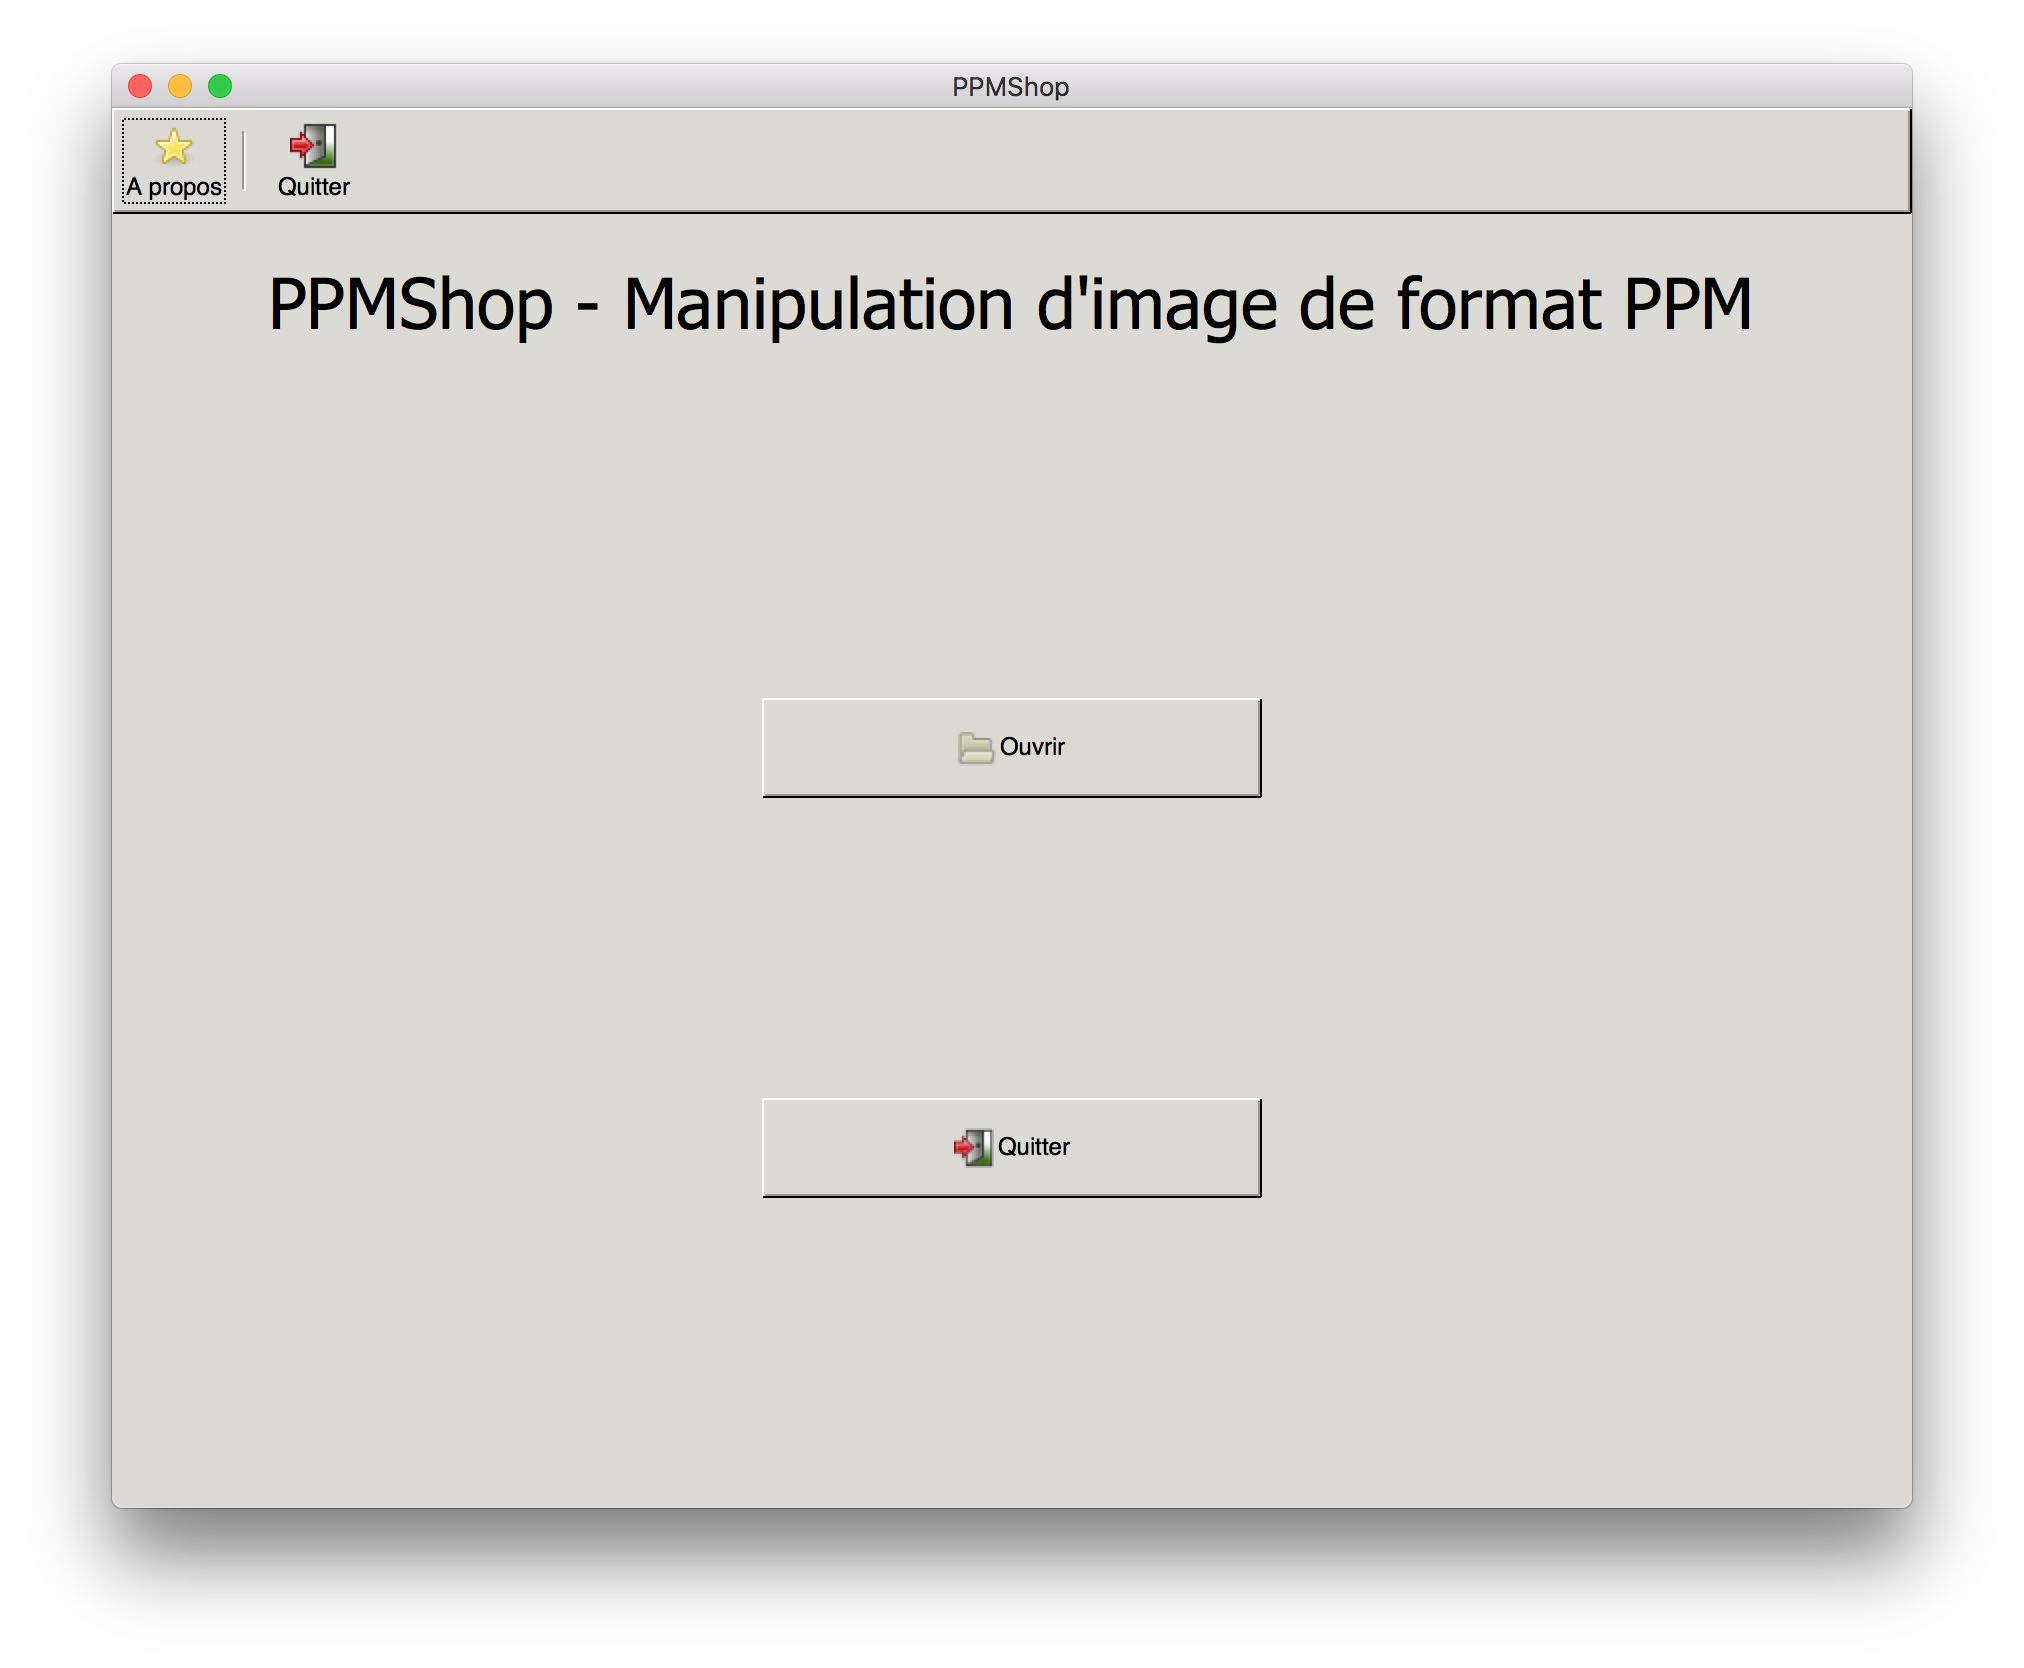
\includegraphics[scale = 0.4]{firstScreen}\\
\end{center}

Il peut ici choisir entre avoir plus d'ample informations sur l'application \textit{PPMShop}, quitter l'application et charger une image.
Si l'utilisateur appuie sur le bouton \textit{À propos}, cet écran sera affiché: 

\begin{center}
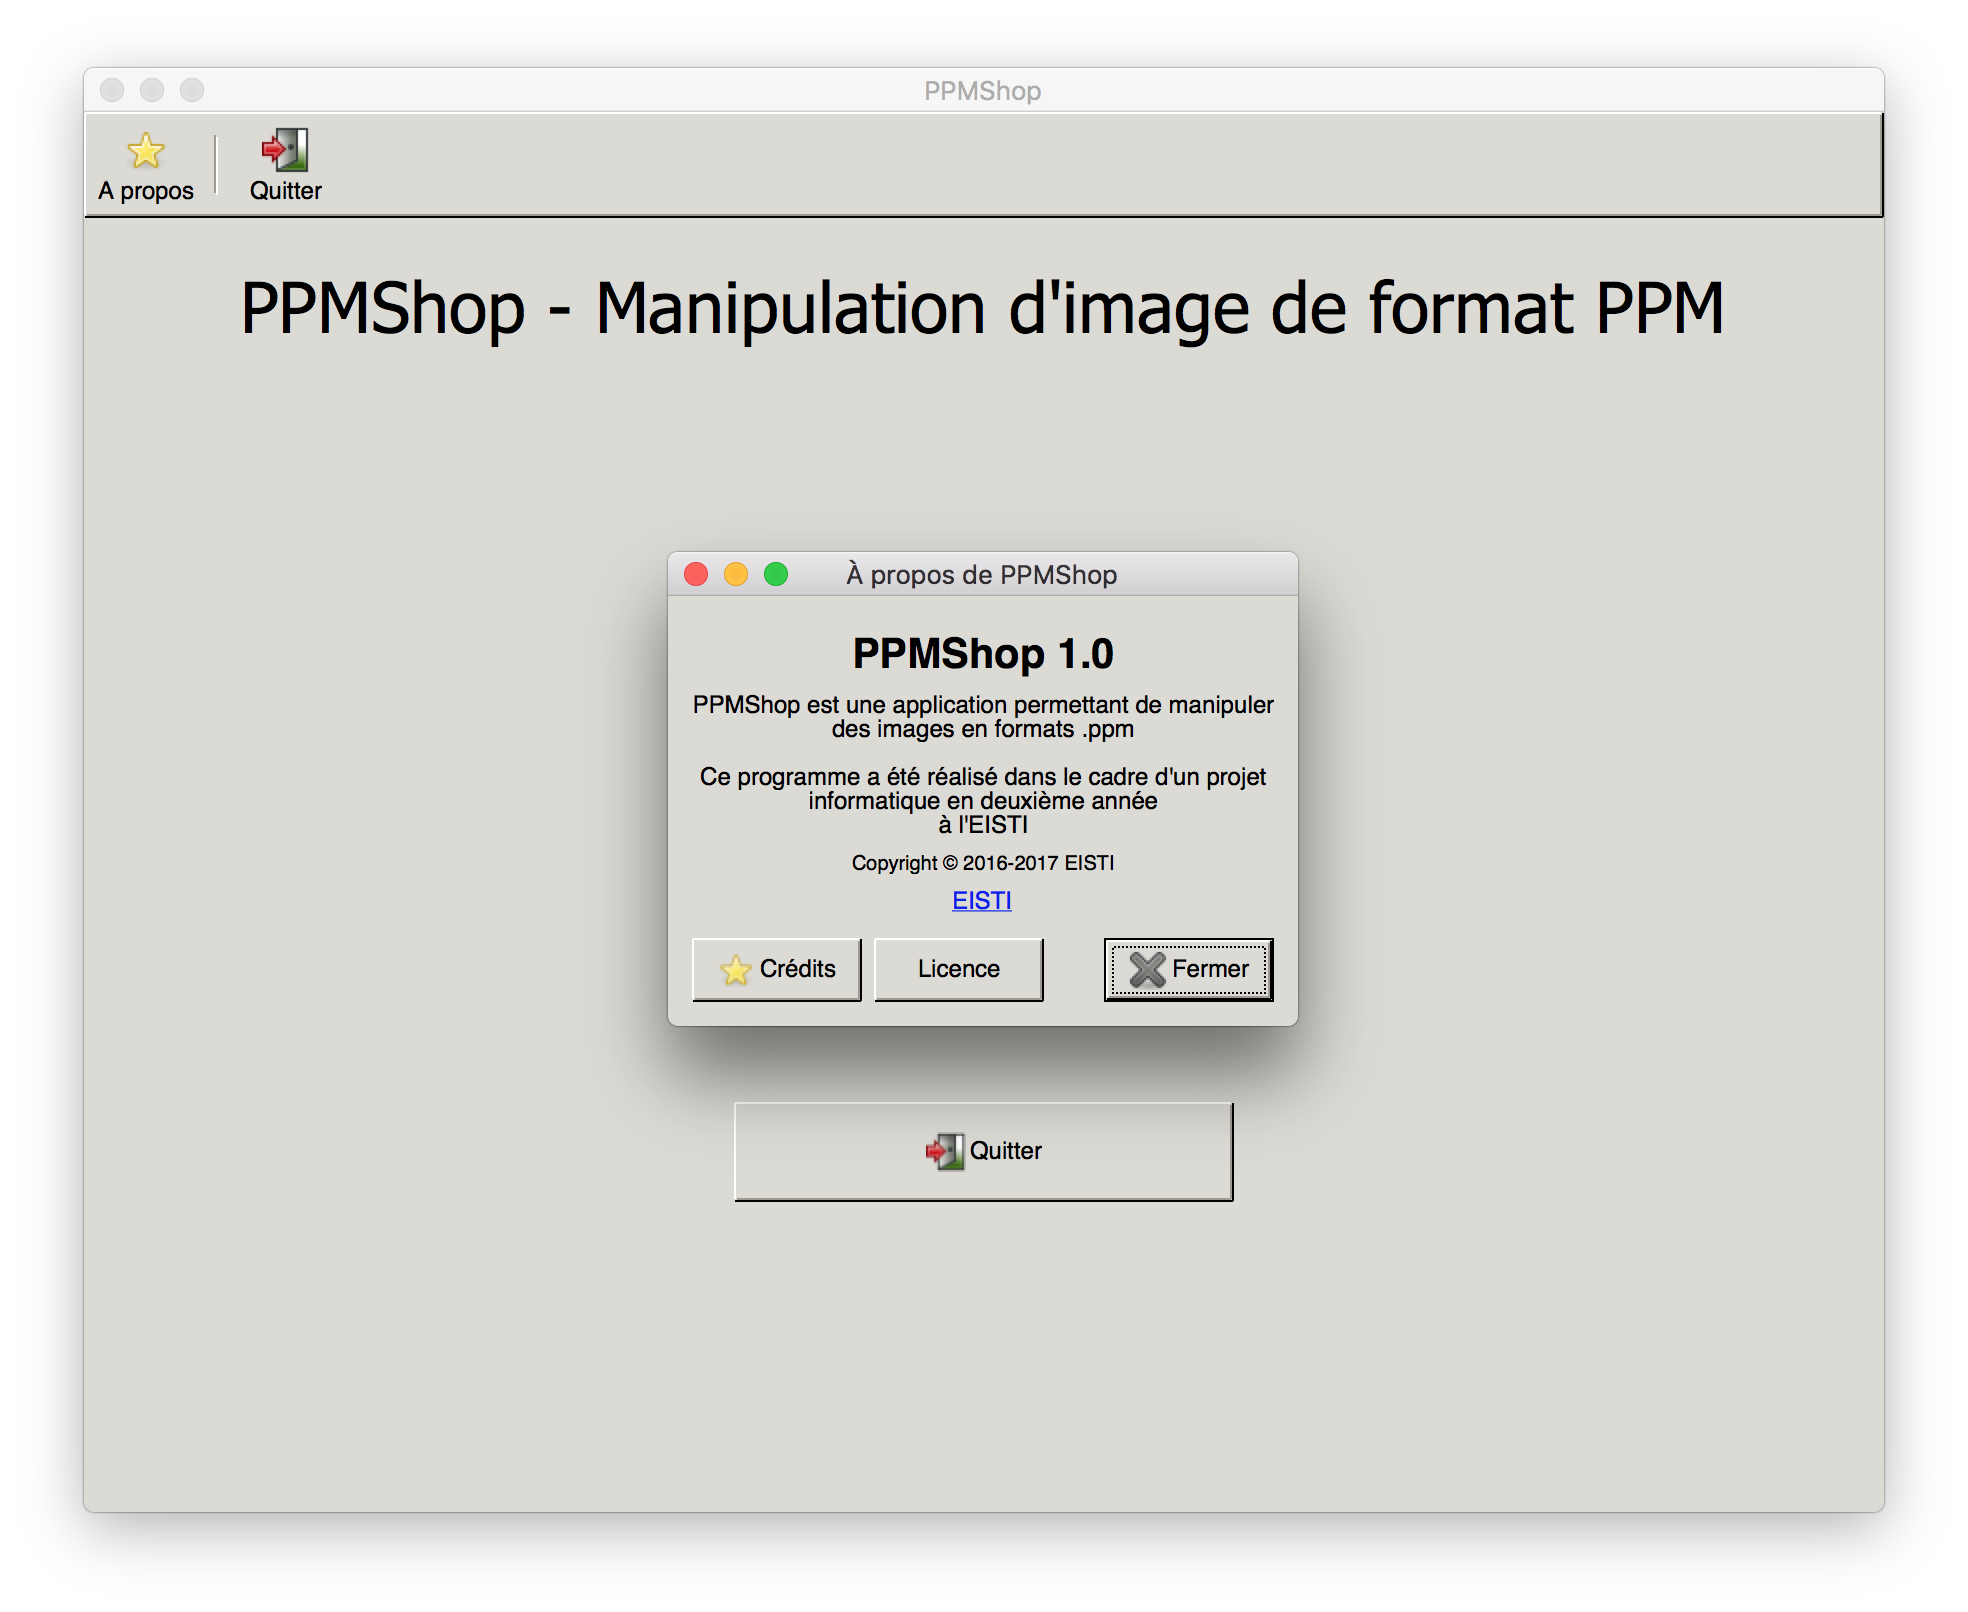
\includegraphics[scale = 0.4]{aboutScreen}\\
\end{center}

Maintenant s'il préfère commencer à vraiment utiliser \textit{PPMShop} et ainsi charger une image en appuyant le bouton \textit{Ouvrir} la fenêtre suivante s'ouvrira : 

\begin{center}
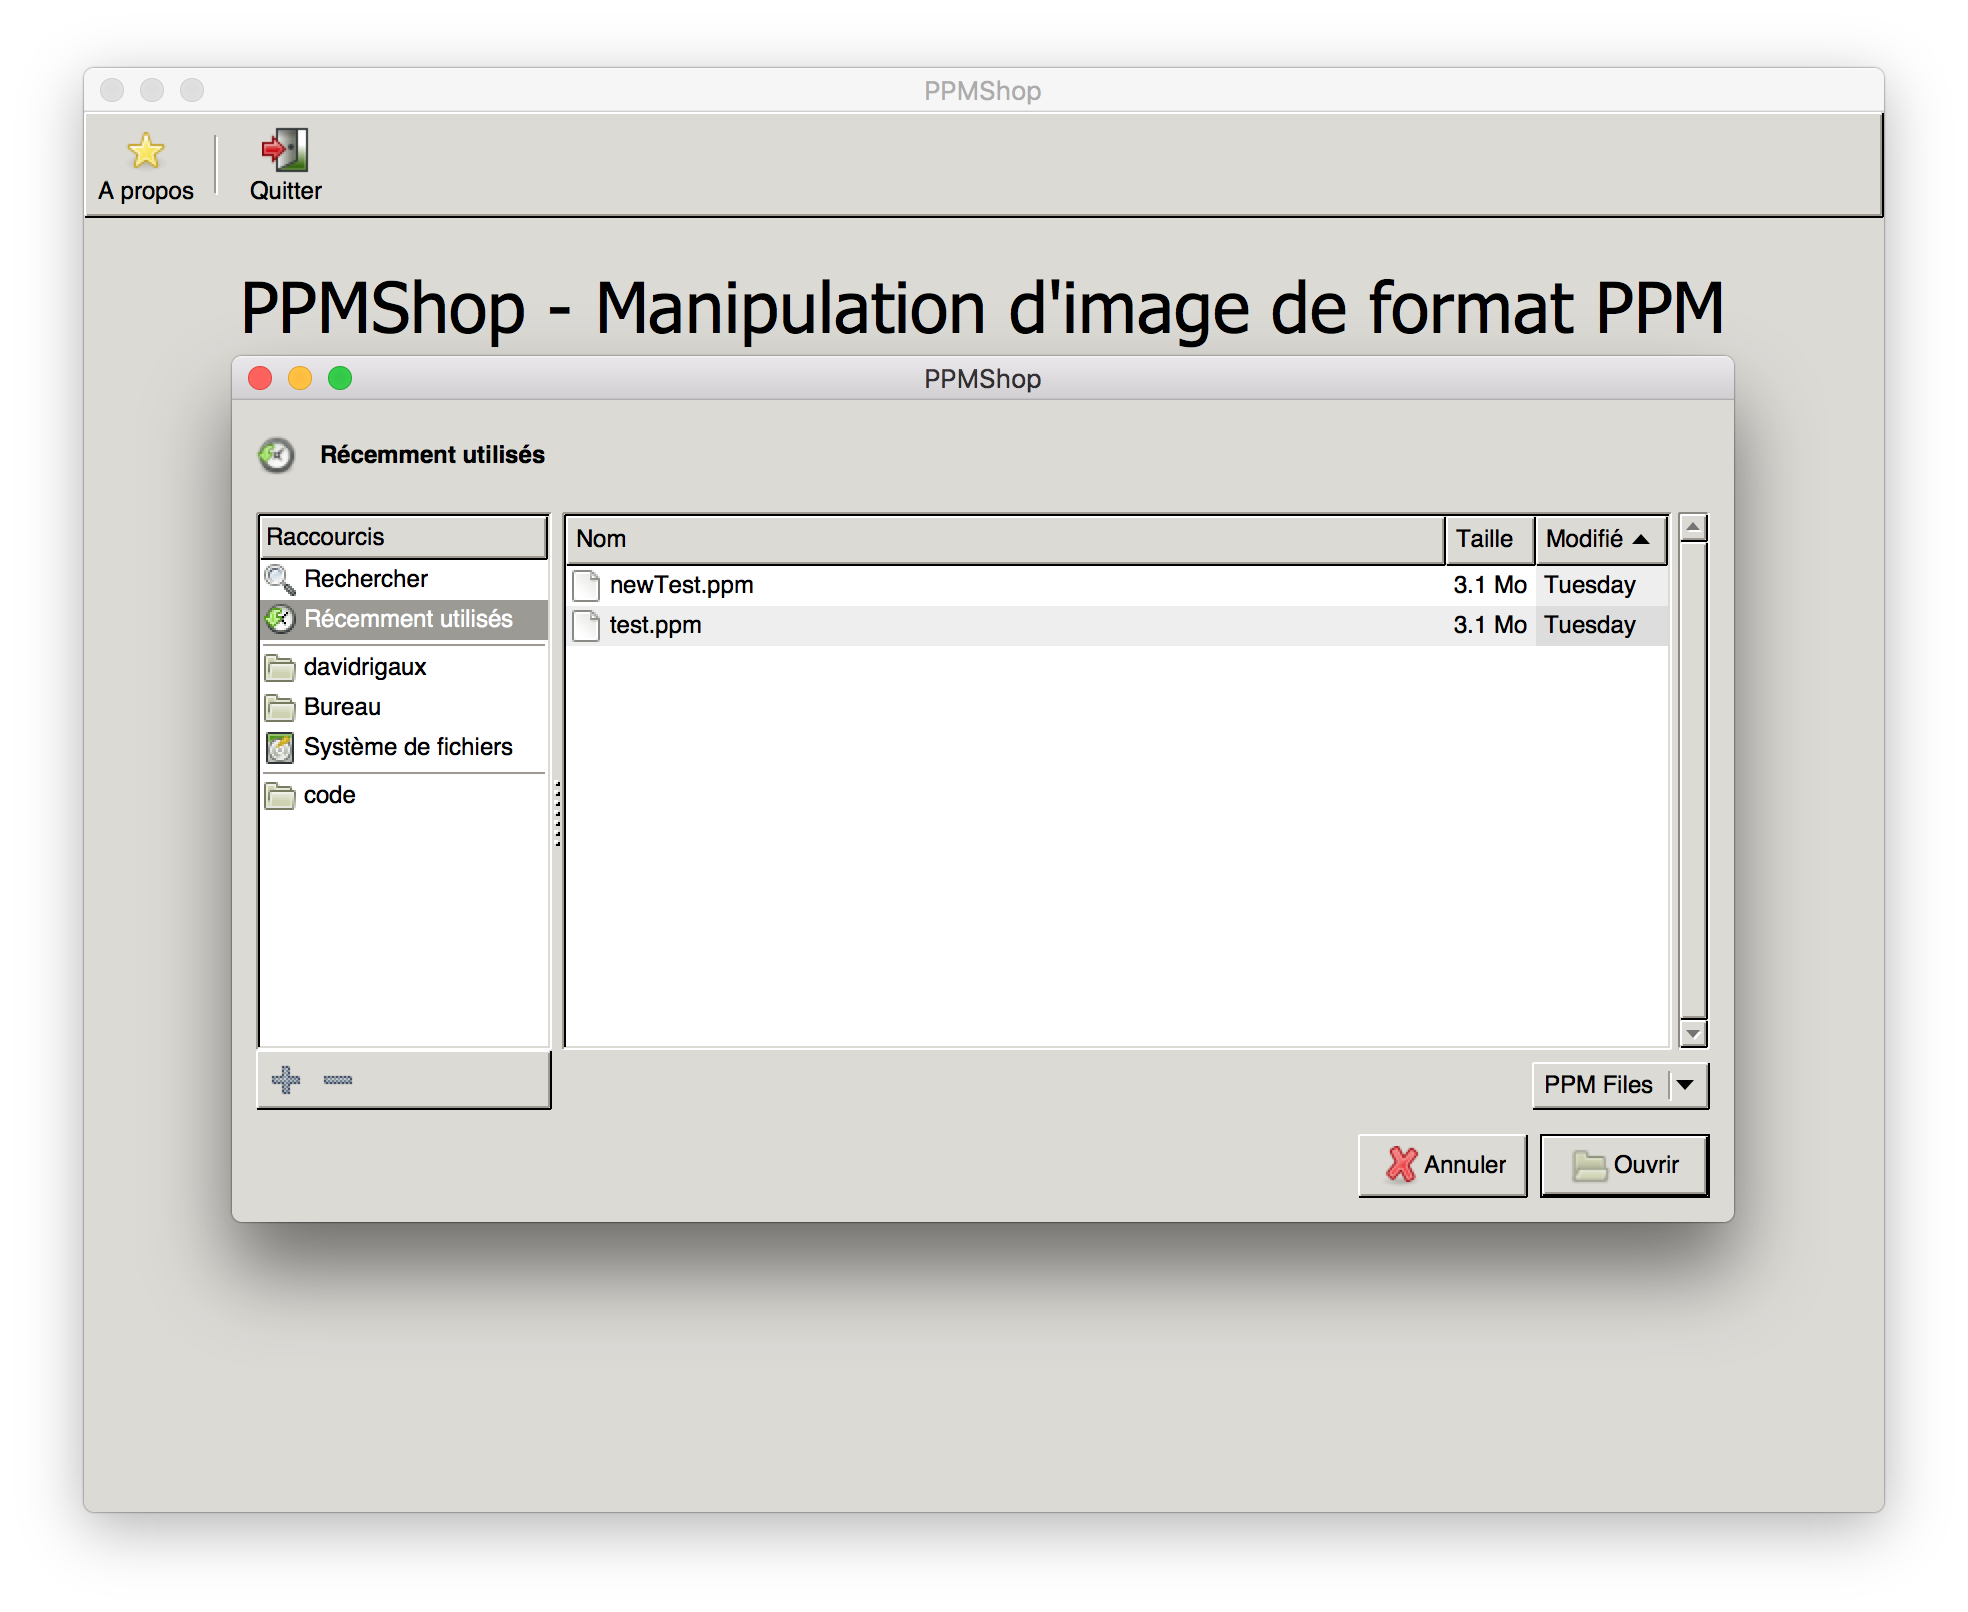
\includegraphics[scale = 0.4]{loadScreen}\\
\end{center}

Ici il pourra alors naviguer parmi tout les fichiers présent sur son ordinateur et ainsi choisir son image en format \textit{.ppm}. On peut également remarquer que dans la partie inférieur droite de cette fenêtre nous avons rajouté un filtre pour les fichiers qui permet d'afficher que les fichiers ayant une extension \textit{.ppm}.
Après avoir choisis son fichier, nous affichons un écran de confirmation d'image ce qui nous permet aussi de faire des vérifications sur l'image choisie (dimensions carrées du fichier, d'extension \textit{.ppm} et de format \textit{\textbf{P3}}).

\begin{center}
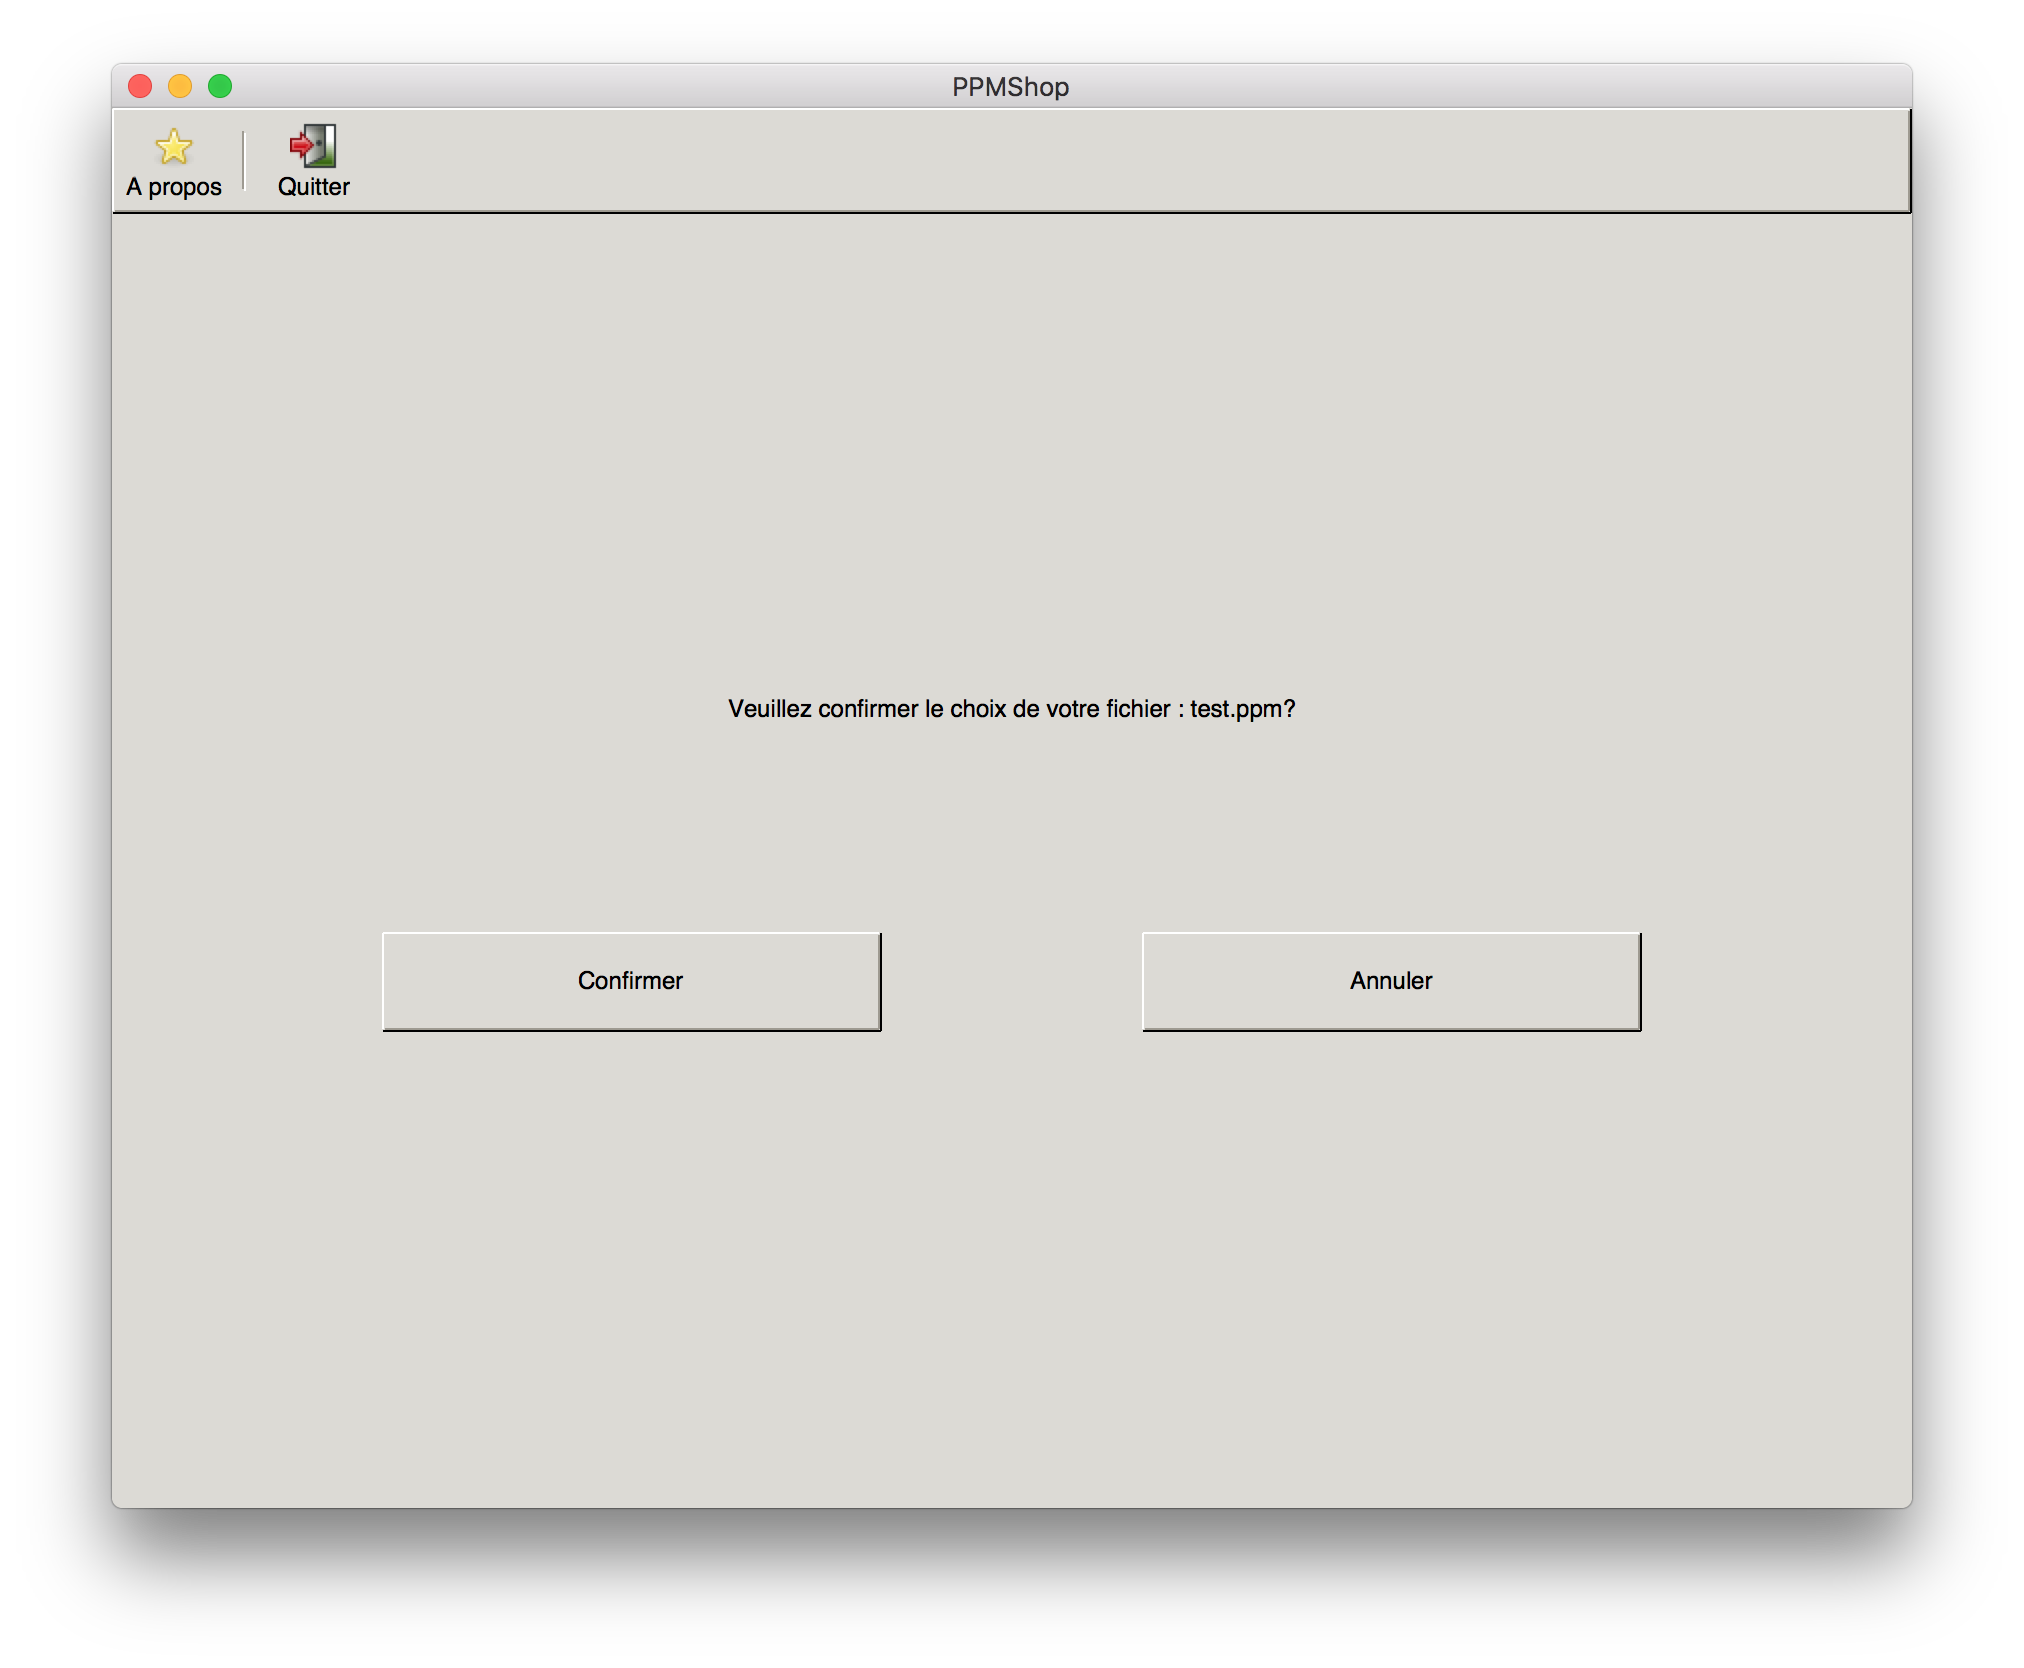
\includegraphics[scale = 0.4]{confirmationScreen}\\
\end{center}

Une fois les vérifications passées et le choix du fichier confirmé le programme affichera son écran principal. Notre programme ayant plusieurs interface possible, il commence systématiquement par afficher la \textit{View 1}, qui correspond à l'interface par défaut.

\begin{center}
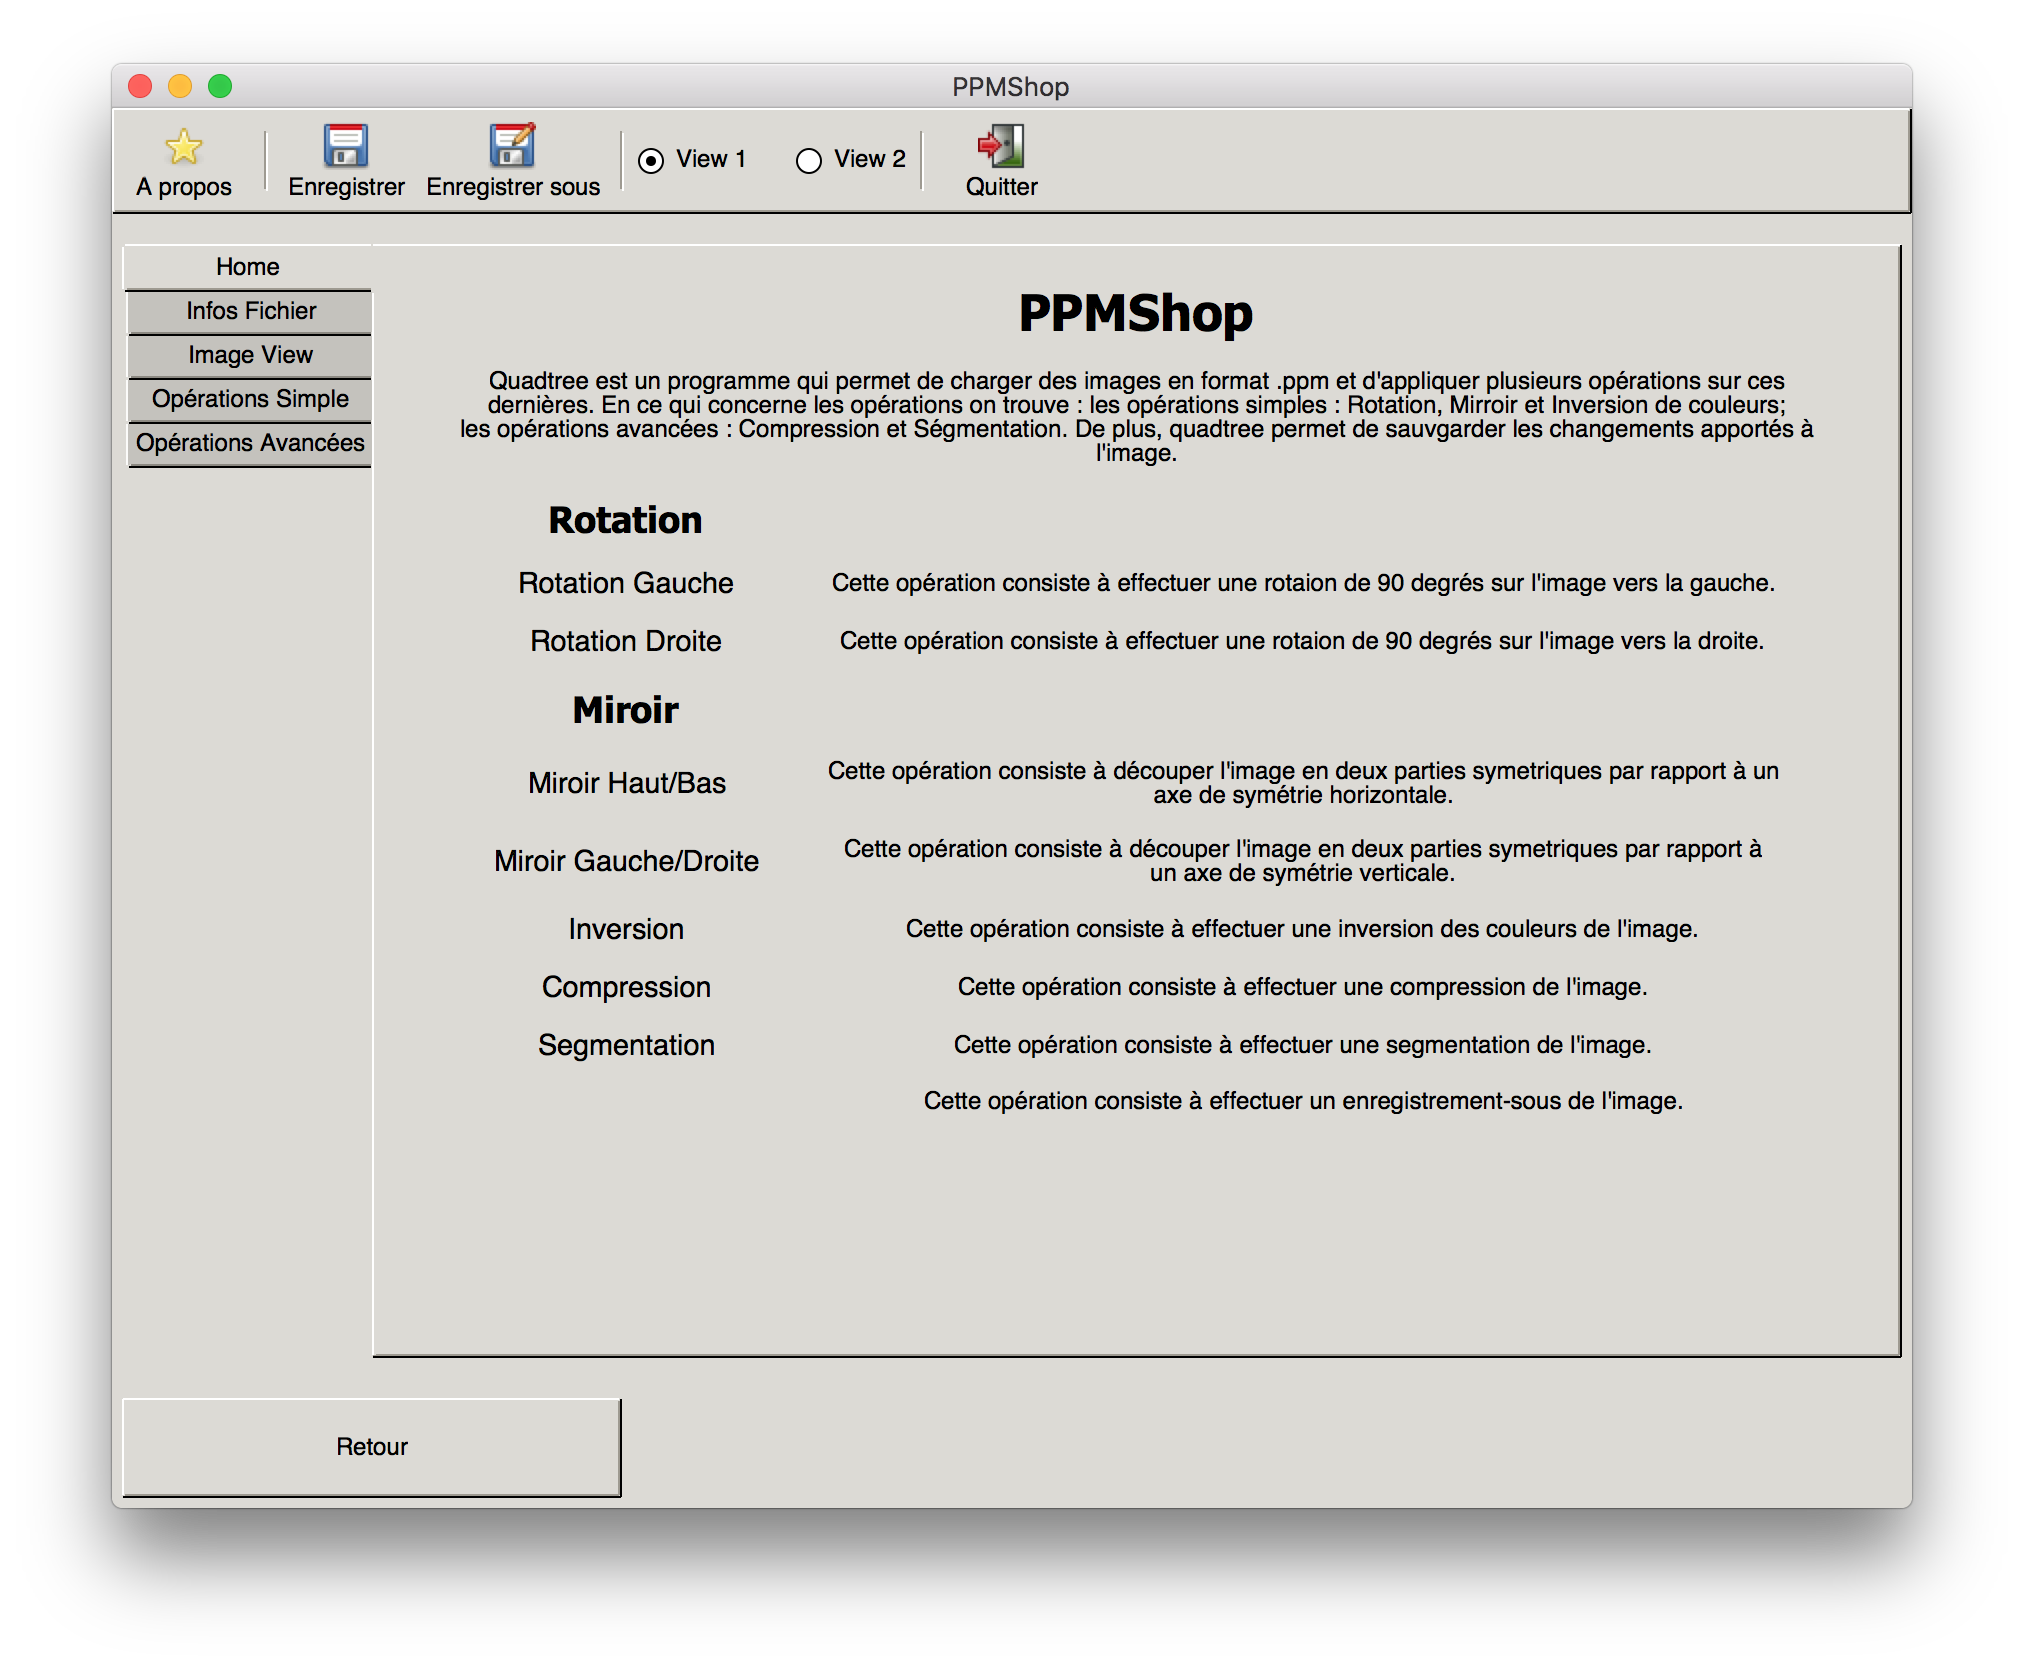
\includegraphics[scale = 0.4]{homeView1}\\
\end{center}
Nous avons ici, accès à toute les informations par rapport à l'image, que ce soit ces dimensions, son nom, un affichage de la photo dans son état actuel, et la possibilité d'appliquer les opérations simples et avancées. 
\subsection{View 1}
Dans la \textit{View 1}, nous avons décidé d'utiliser des onglets qui affiche les informations et les boutons que l'on souhaite avoir ou utiliser. 
\begin{center}
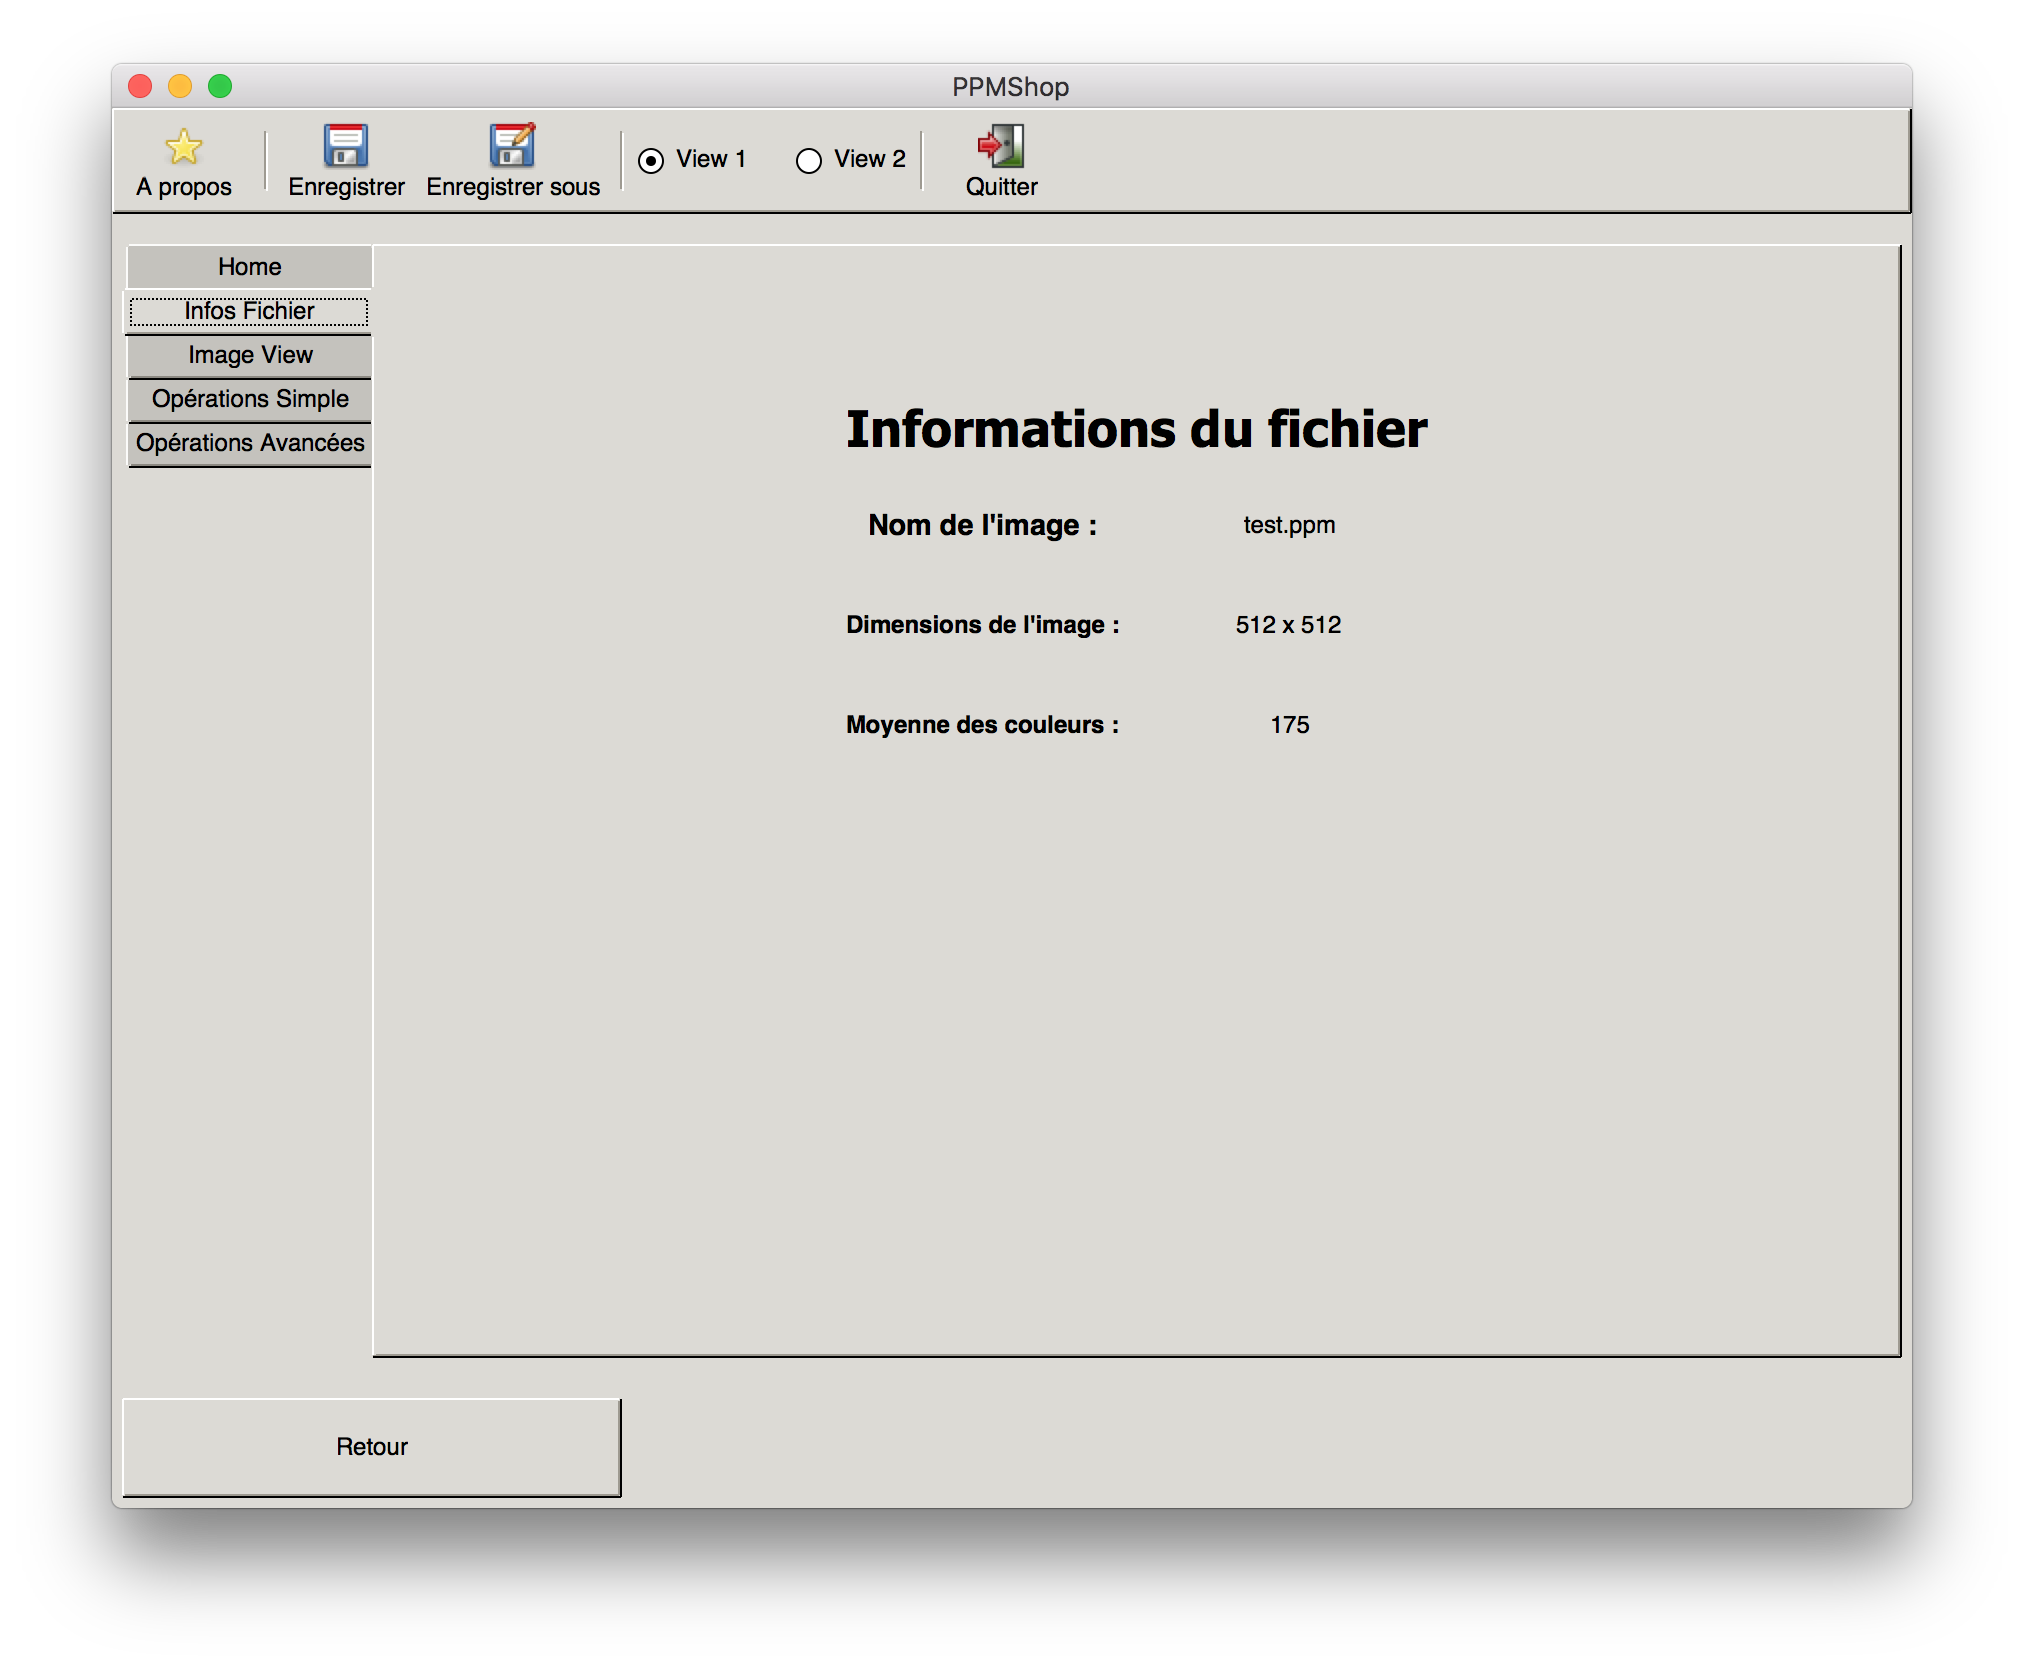
\includegraphics[scale = 0.3]{infosView1}\\
\end{center}
\begin{center}
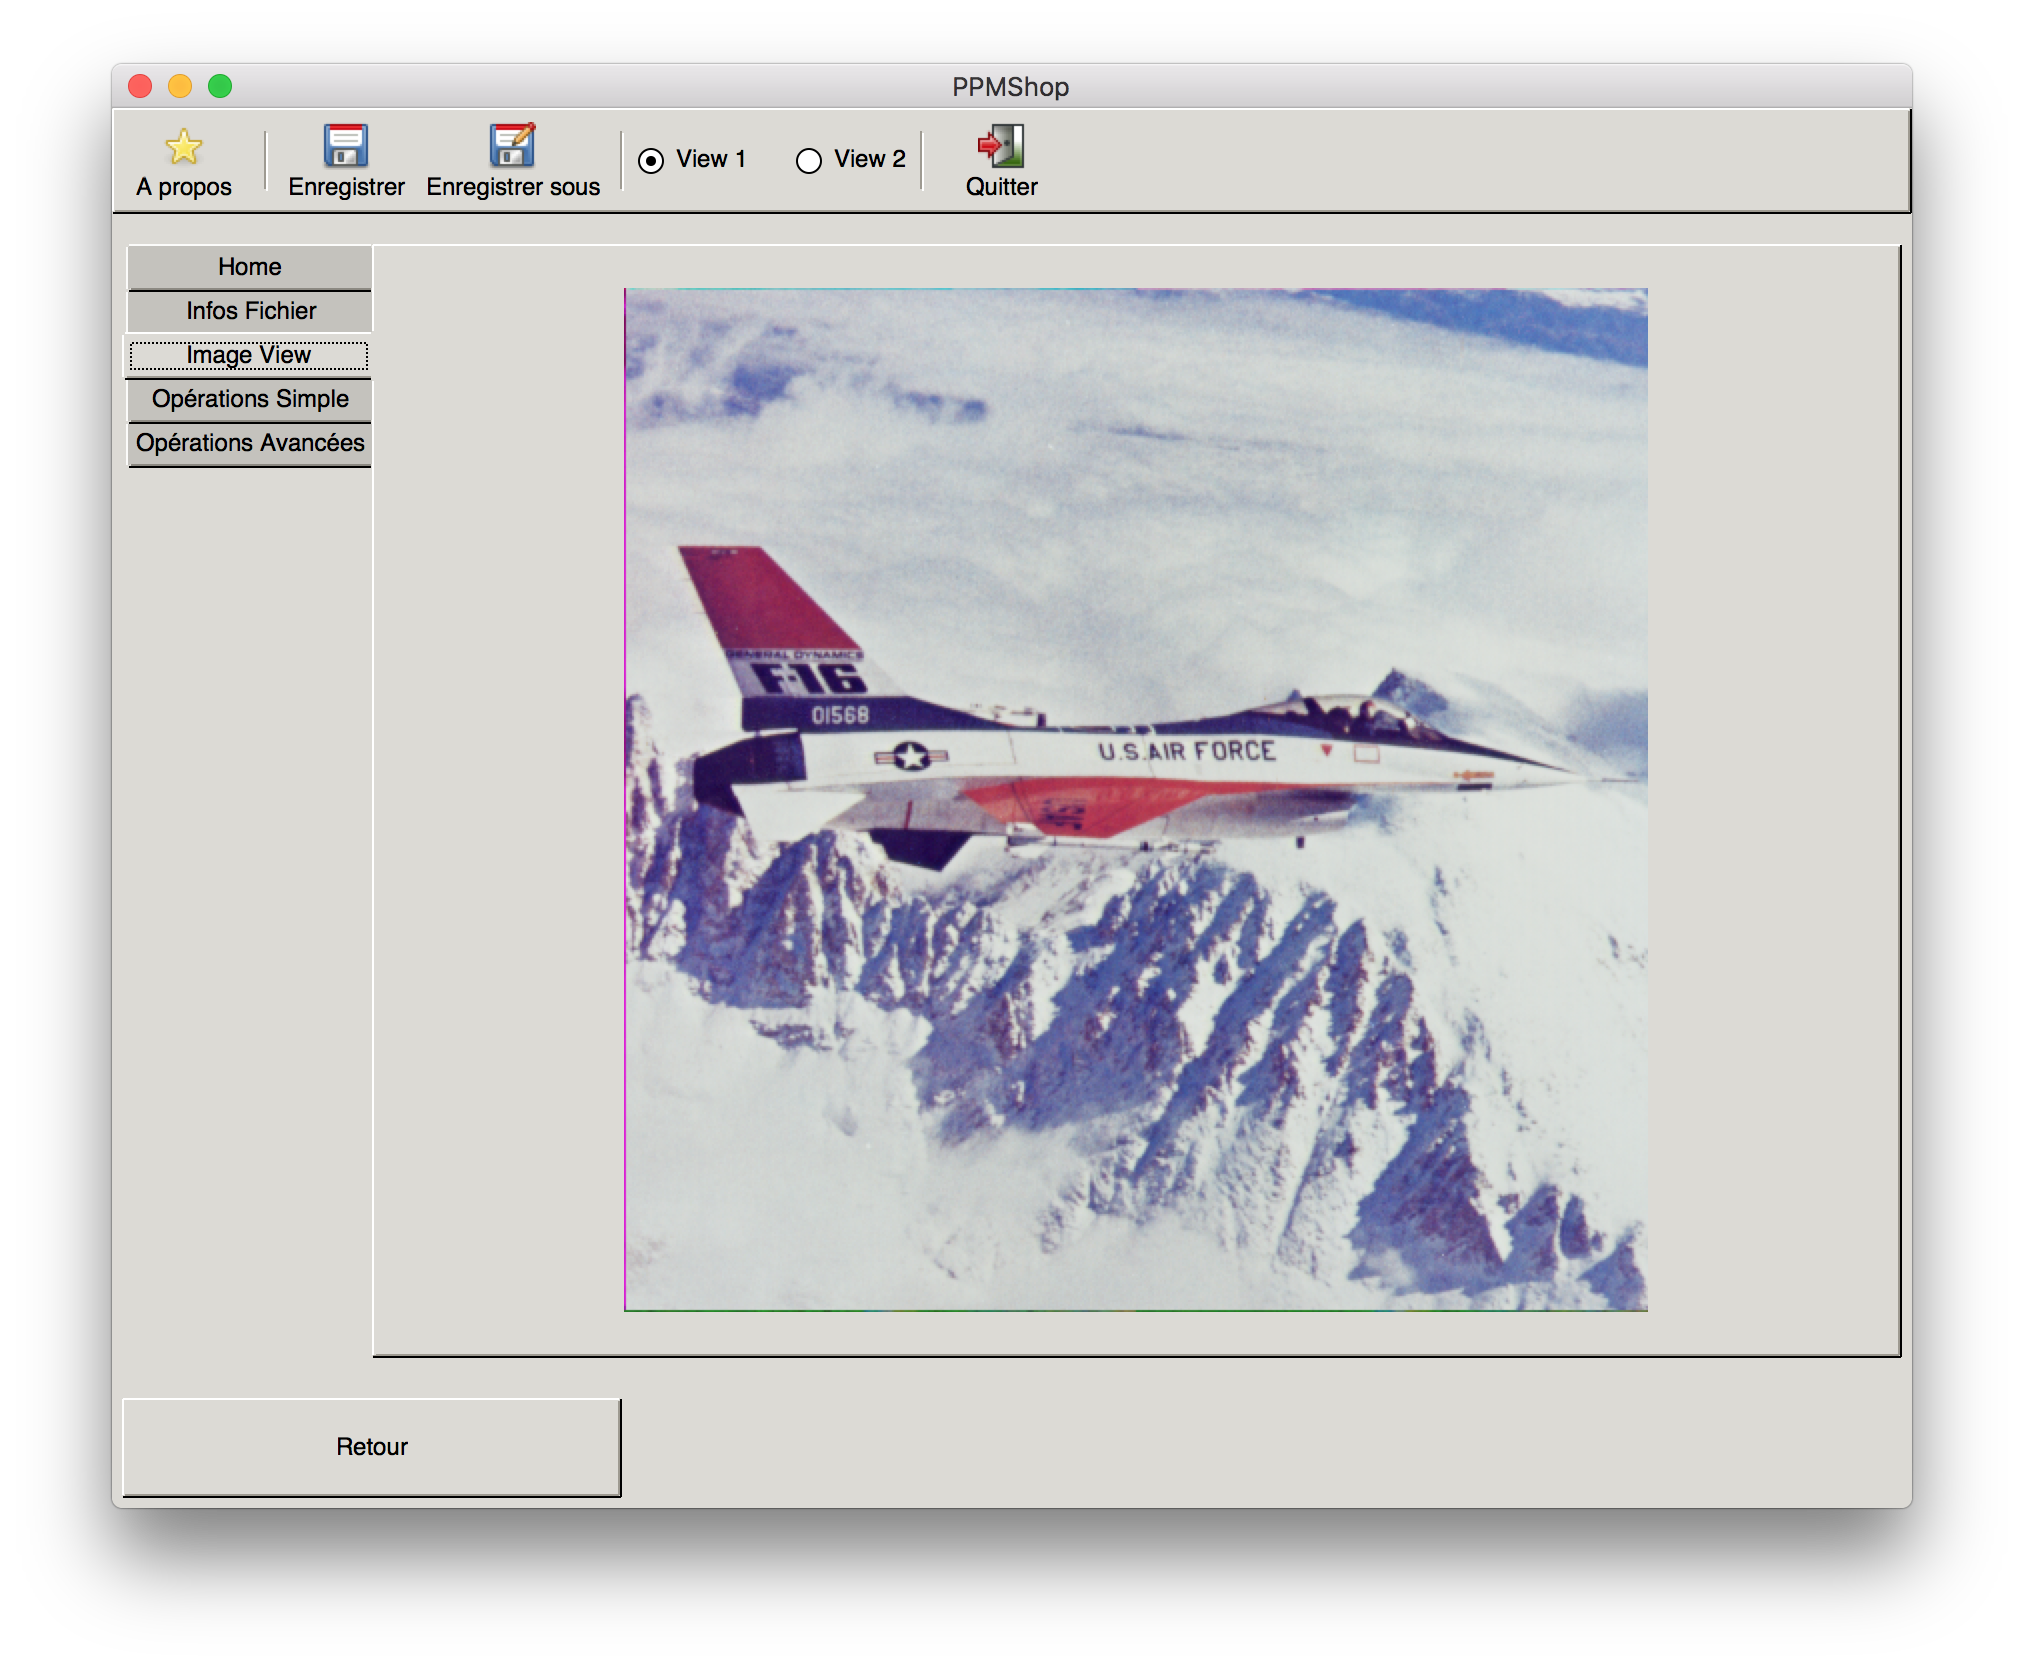
\includegraphics[scale = 0.3]{imageView1}\\
\end{center}
\begin{center}
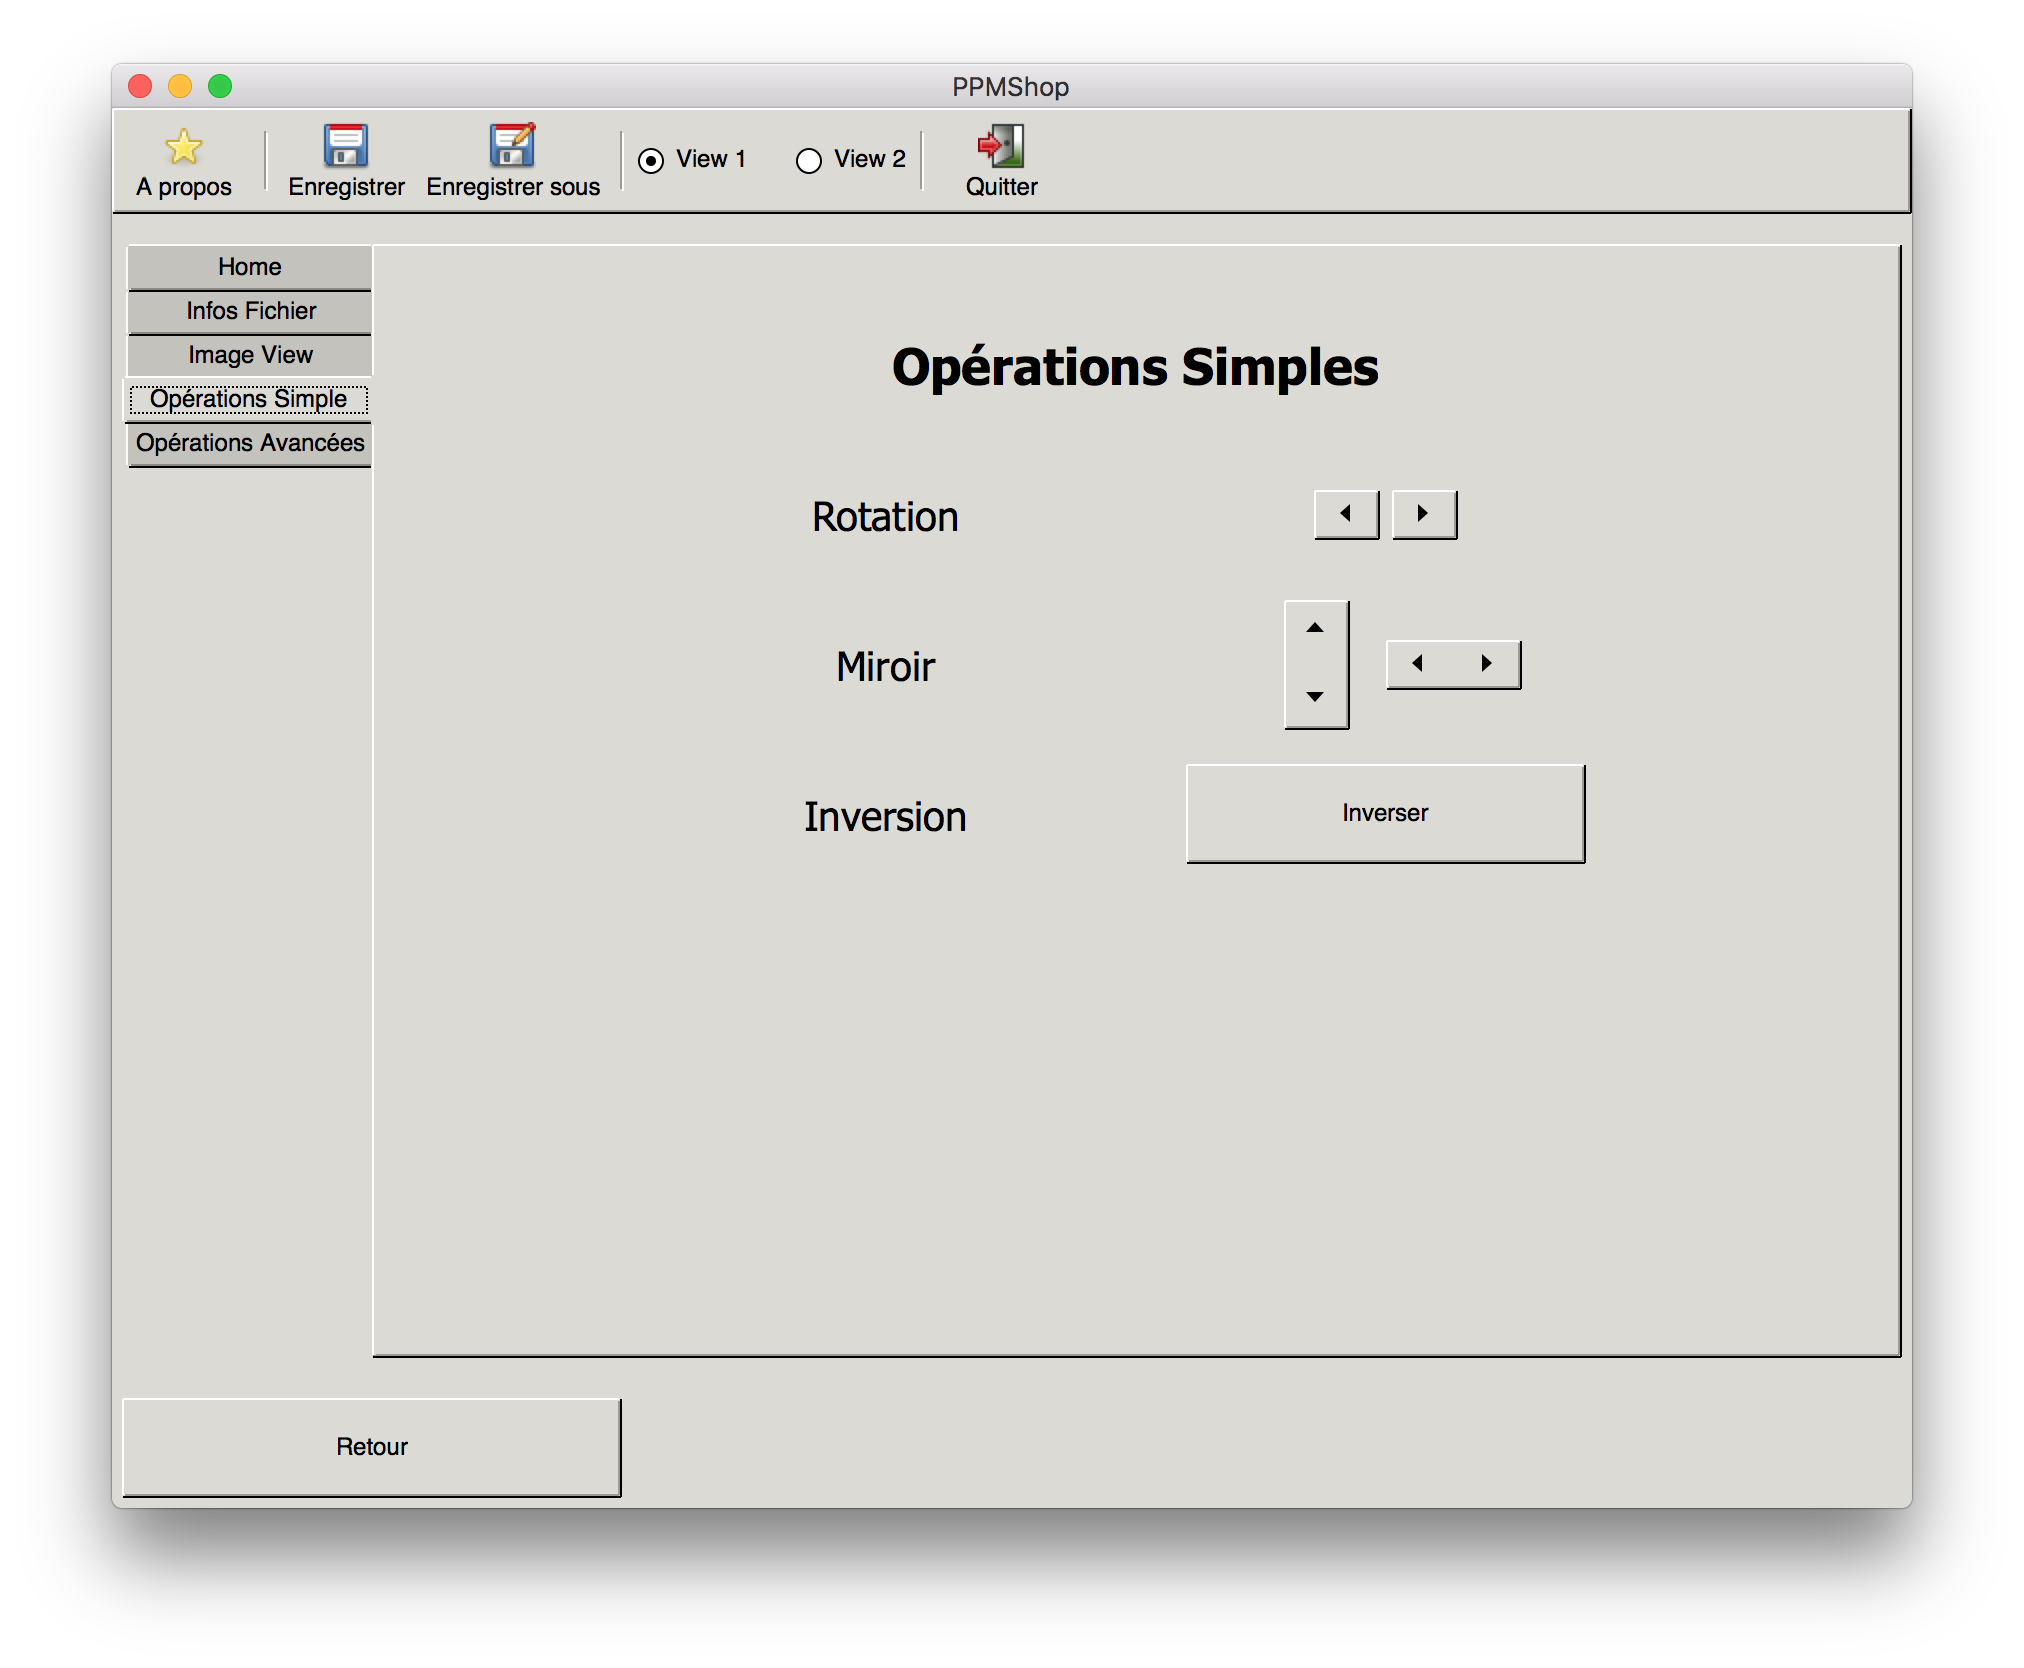
\includegraphics[scale = 0.3]{opeSimpleView1}\\
\end{center}
\begin{center}
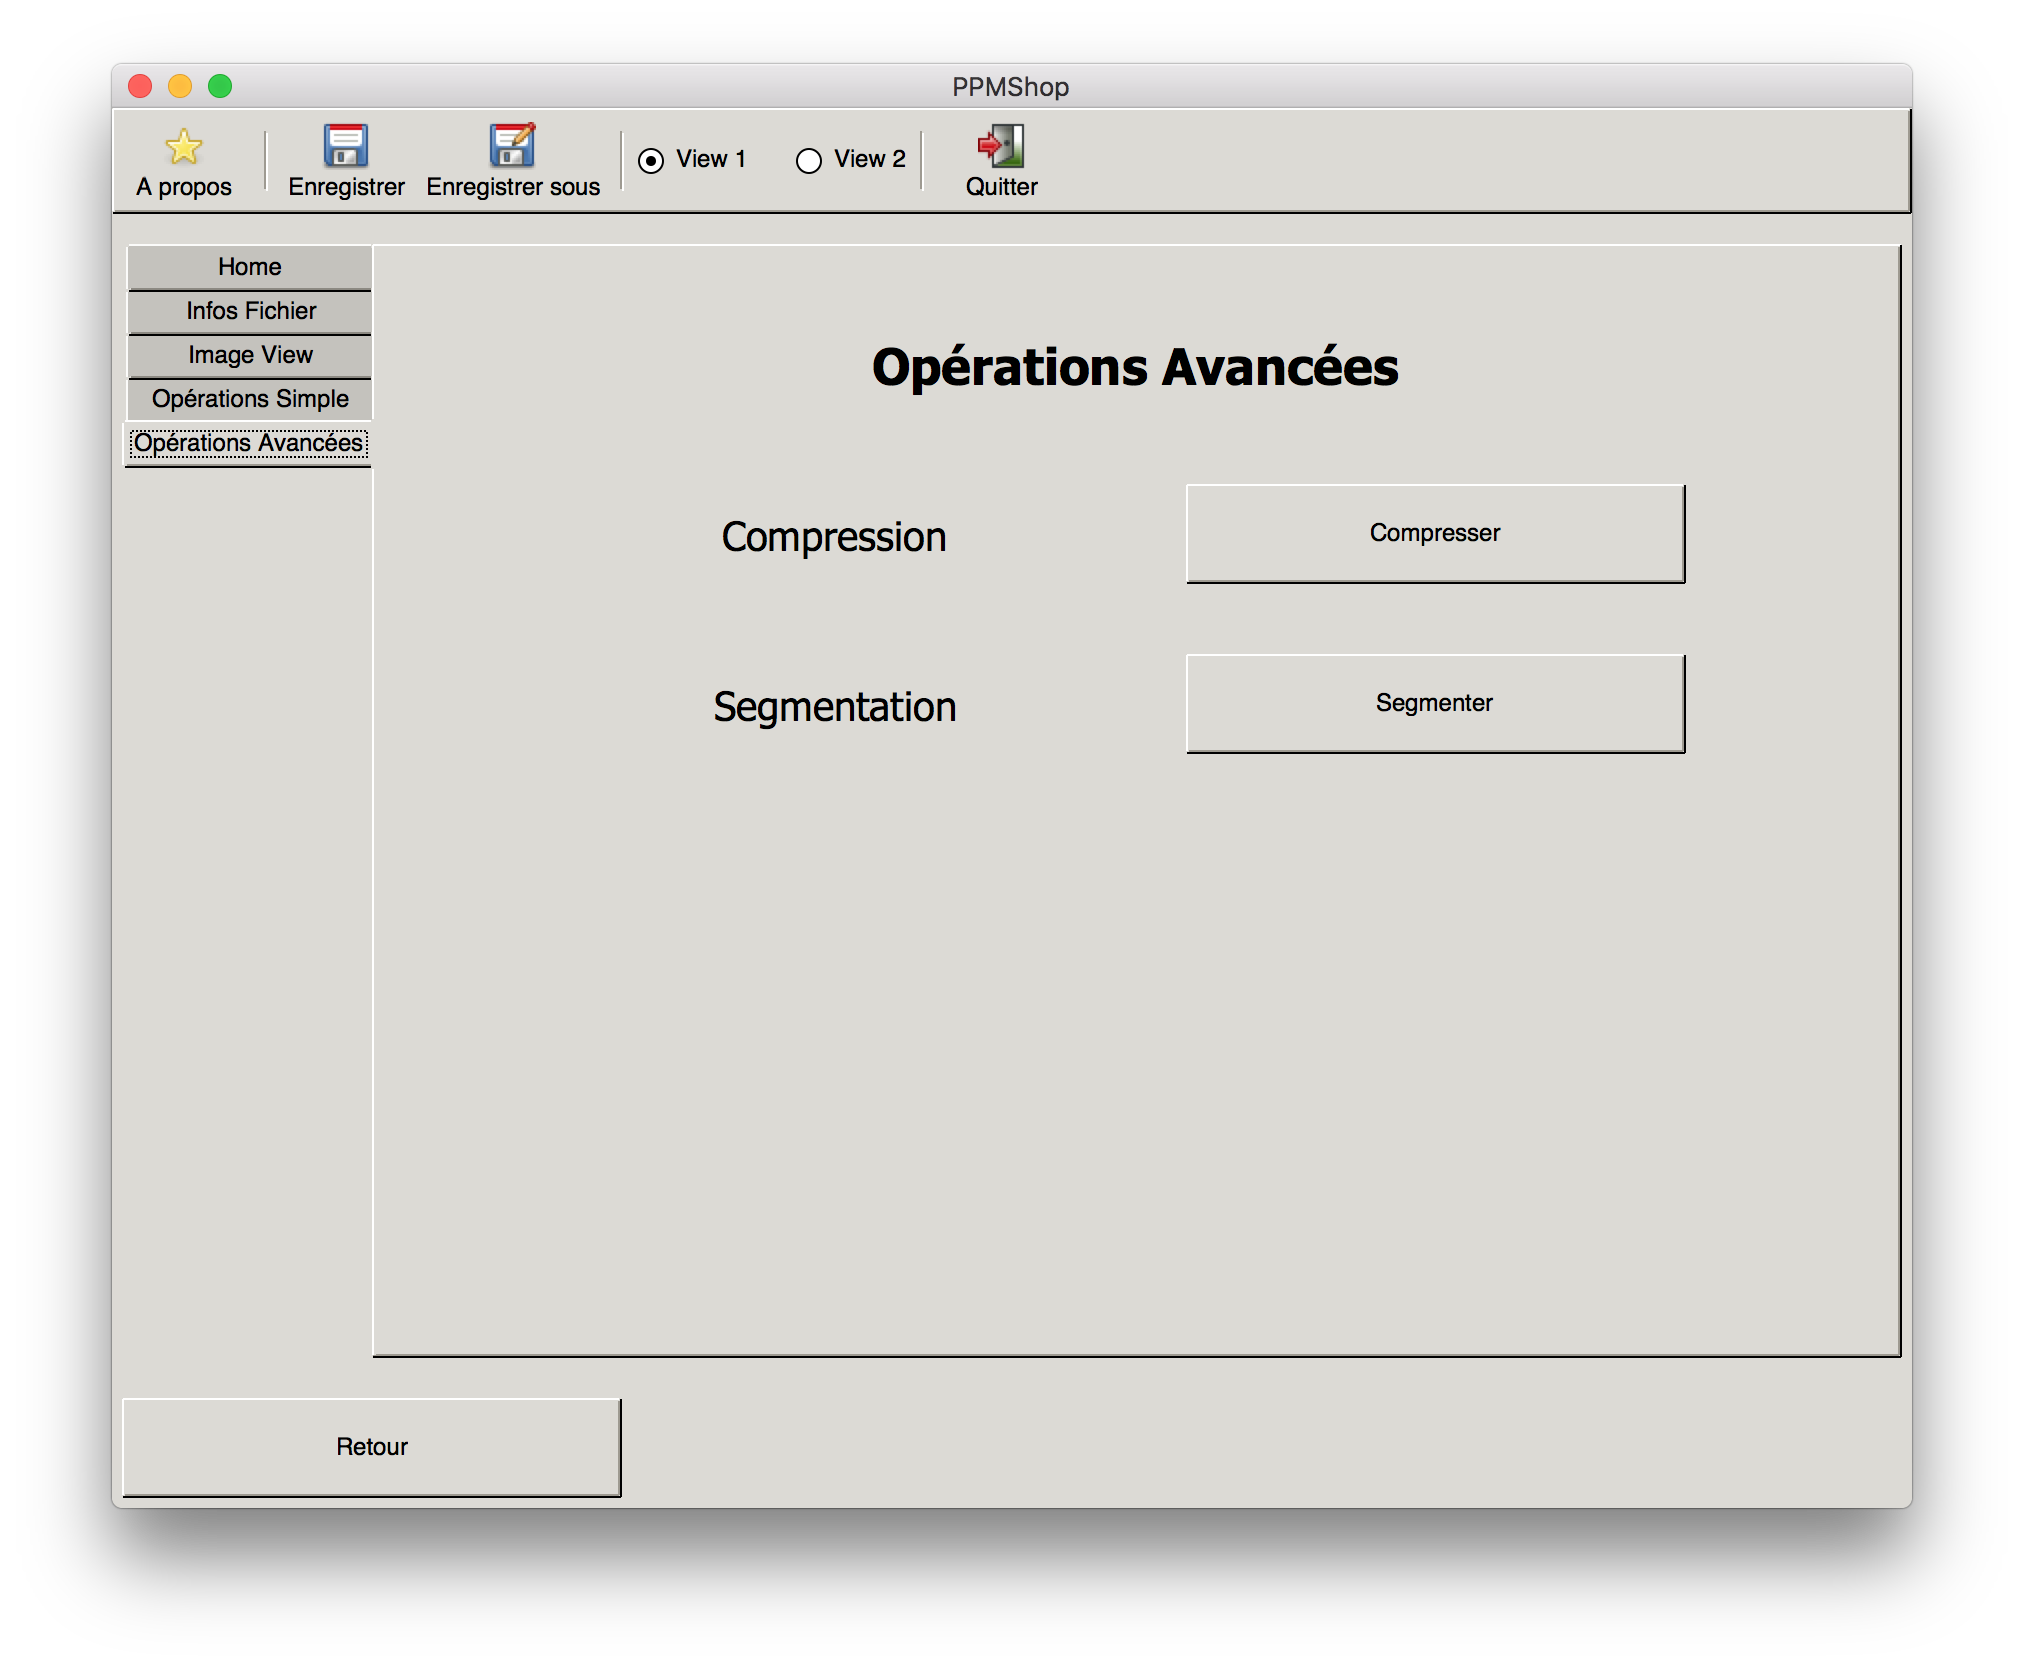
\includegraphics[scale = 0.3]{opeAdvView1}\\
\end{center}
Si l'utilisateur préfère utiliser la \textit{View 2}, il lui suffit d'appuyer sur le bouton radio qui se situe sur la barre à outils sur la partie supérieur de l'application. Celle-ci ressemble à ceci :\\
\begin{center}
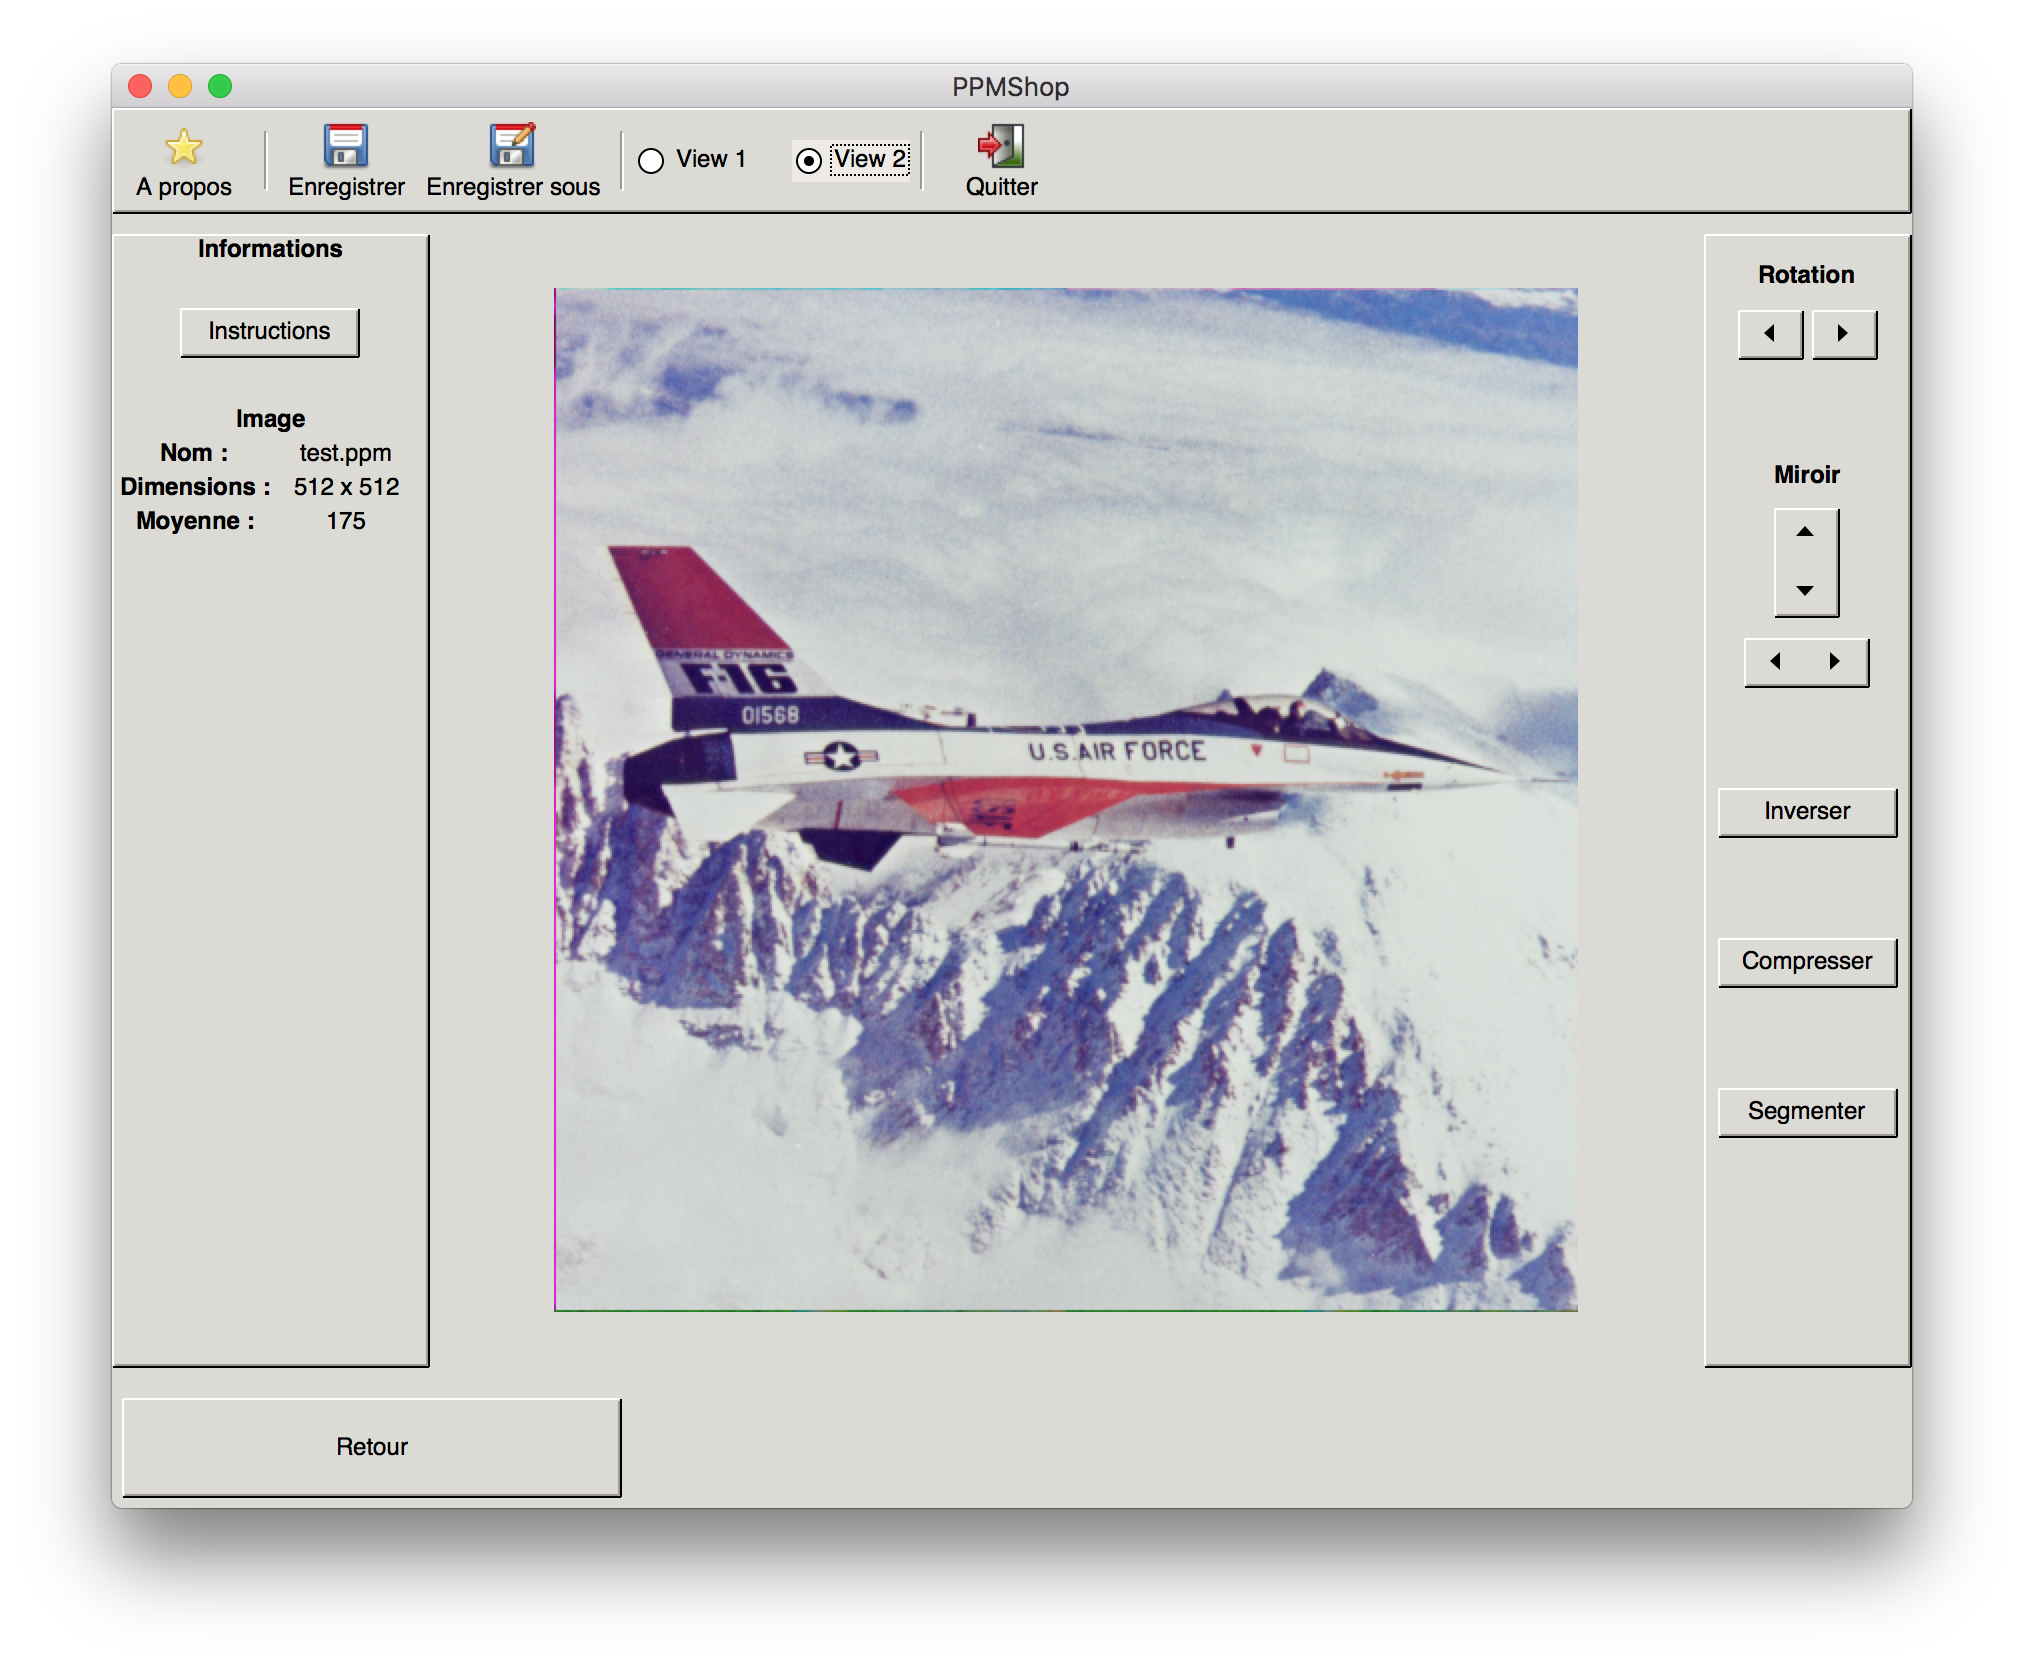
\includegraphics[scale = 0.3]{view2}\\
\end{center}
Qui est une vue plus compacte, qui donne accès à toute les fonctionnalités sur un écran et la possibilité de voir le changement de l'image en temps réel. 
\section*{Conclusion}
\addcontentsline{toc}{section}{\protect\numberline{}Conclusion}
\end{document}
